\documentclass[../labs.tex]{subfiles}

\pagestyle{main}
\renewcommand{\leftmark}{\large Lab Report \thesection}
\fancyhead[R]{\large CHEM 26700}
\fancyfoot[R]{\large Labalme \thepage}
\setcounter{section}{5}

\begin{document}




\large
\captionsetup[figure]{labelfont={bf},labelsep=period}



\noindent Steven Labalme\\
TA: Ben Masters\\
Lab partners: Joe Geniesse, Irene Madejski, and Sophia Madejski\\
16-23 February 2023\hfill
2 March 2023

\section{ANALYSIS OF THE ELECTROCATALYTIC ACTIVITY OF PLATINUM, TIN, AND TITANIUM TOWARD THE HYDROGEN EVOLUTION REACTION}
\subsection*{Abstract}
% Goals: hi
% Results: hi
% Takeaways: hi

% This experiment uses the hydrogen evolution reaction, known as HER, which allows for non-carbon-based energy storage. In the experiment, cyclic voltammetry and chronoamperometry were performed to determine a rate law for the HER. The chronoamperometry data collected allowed for the calculation of which mechanism is present for each of the electrodes. It was concluded that the HER with the platinum reaction functions by the Volmer-Tafel mechanism, while titanium and tin function via the Volmer-Heryovsky mechanism. The rate law for the HER is concluded to be dependent on the binding energetics of the key reaction intermediates to the electrocatalyst surface. More specifically, the metal hydride bond strength serves as an indicator of the rate of the HER. Overall, this experiment serves to provide the tools necessary to design an efficient electrocatalyst.

The goal of this experiment is to evaluate three candidates for the electrocatalysis of the hydrogen evolution reaction (a reaction in which there is broad chemical and societal interest), and to probe the mechanism over each of metal to determine which of two well-defined types is active. It was determined that the order of catalytic activity is platinum, then titanium, then tin. Additionally, it was determined that platinum follows the Volmer-Tafel mechanism with second-order reaction kinetics in the concentration of acid, and tin follows the Volmer-Heyrovsky mechanism with first-order kinetics in said concentration. Altogether, the data suggests that the metal-hydride bond strength is a key indicator of the rate of the hydrogen evolution reaction, providing a key tool necessary to design future reactions.

% \textbf{TRANSITIONS BETWEEN SECTIONS}


\subsection*{Introduction}
\onehalfspacing
% Tips: Funnel approach, clear, short, not too many equations (but don't leave stuff out), don't be repetitive.
% When introducing new variables: Include units, state what they mean, state relation to molecular behavior.

% Broad questions and motivation:
% \begin{itemize}
%     \item Electrochem has the potential to solve important problems in synthesis, renewable energy, energy storage, etc.
%     \begin{itemize}
%         \item \ce{CO2}RR could store energy by using wind or solar to drive this electrochemical reaction.
%         \item Increasing energy demand and climate change drive the need for a sustainable future \emph{cite seh paper}
%     \end{itemize}
%     \item Electrochem is particularly interesting because it is very easy to probe mechanisms, a rarity in chemistry.
%     \begin{itemize}
%         \item Example: You always know the rate; the velocity is proportional to the easily measured current.
%     \end{itemize}
%     \item Mechanisms being well understood means that rational design is highly feasible.
%     \begin{itemize}
%         \item Example: Electrochem presents a possible alternative to upconversion of \ce{CO2} and other simpler carbon compounds outside of the water-gas shift reaction and Fischer-Tropsch chemistry. Has been partially realized with the production of ethylene from \ce{CO2 + H2O}.
%     \end{itemize}
%     \item Why is the HER cool?
%     \begin{itemize}
%         \item It's got a very simple mechanism, but also one that reveals a lot; for example, hydrogens are often added to the surface not from solution (hydronium) but from acid molecules themselves such as carbonic acid. Reveals subtelty but problem-solving power of electrochemistry.
%         \item REWRITE DON'T PLAGARIZE: The HER is a classic example of a two-electron transfer reaction with one catalytic intermediate, and offers the potential to produce \ce{H2}, a critical chemical reagent and fuel.
%         \item Cite Jin paper!
%     \end{itemize}
%     \item Selectivity is still a big issue, though.
%     \begin{itemize}
%         \item In Fischer-Tropsch chemistry, we can improve it by acting on a better understanding of the catalytic surface and knowing that a mesoporous membrane will help; \emph{cite Wuttig paper}!
%     \end{itemize}
%     \item How can we enhance selectivity in the HER?
%     \begin{itemize}
%         \item Get molecular level insight into the reaction mechanism first.
%         \item One way is to make sure we use the best catalytic electrode material possible. Correlation with surface metal-hydride bond strength.
%         \item Transition metals are natural candidates because their incompletely filled $d$-orbitals make them good (not rigid) donors and acceptors of electrons.
%     \end{itemize}
% \end{itemize}
% Objective.
% Purpose:
% \begin{itemize}
%     \item How does CV help?
%     \begin{itemize}
%         \item CV allows us to identify the region in which catalysis begins.
%     \end{itemize}
%     \item How does CA help?
%     \begin{itemize}
%         \item CA allows us to extract data that will allow us to construct a Tafel plot.
%     \end{itemize}
%     \item How do Tafel plots connect experimental data to molecular level insight?
%     \begin{itemize}
%         \item Tafel plots have slopes that can differentiate between probable mechanisms.
%         \item The HER only proceeds through two possible mechanisms (V-T) and (V-H).
%         \item Thus, we can use a Tafel plot to tell us which mechanism is accurate, from which we can derive rate law information and most anything else about the system. Molecular-level understanding really is key.
%     \end{itemize}
%     \item What variables and equations do I want to talk about?
%     \begin{itemize}
%         \item Certainly the HER should be in there.
%         \item Correcting for the mercury electrode.
%         \item $j=I/A$ (units \si{\milli\ampere\per\centi\meter\squared}, \si{\ampere} or \si{\milli\ampere}, \si{\centi\meter\squared}). Current density is the amount of electrons flowing through a unit of area in a given amount of time. It is an intensive property. Current is just the net flow of electrons, and area is area.
%         \item CA: $\log(-j)$ (units decades).
%         \item $\eta=E_{\ce{H+/H2}}-E_\text{app}$ (units \si{\volt} or \si{\milli\volt}). Overpotential is the potential past the standard you have to apply to get the HER to run. It reflects the kinetic barriers to a certain metal engaging in catalysis. $E_\text{app}$ is what you actually have to apply. The first $E$ is the standard.
%         \item Tafel slope relation derivation.
%         \item Volmer-Tafel mechanism.
%         \item Volmer-Heyrovsky mechanism.
%     \end{itemize}
% \end{itemize}
% Methods: CV and CA, Excel, linear regression.
% Background and strategy (essential connections between theory and experiment; basic principles for measurement): See above.
% Clear closing statement that summarizes the specific methods and analysis to follow: Write last.

% Using cyclic voltammetry (CV), the maximum anodic current that flows during the potential sweep is correlated with the activity of the catalyst. Although the current $I$ will correlate with activity to an extent, it will be better to use \emph{current density}, defined as follows.
% \begin{equation}
%     j = \frac{I}{A}
% \end{equation}
% Current density is an \emph{intenstive} property of the given metal and is thus a better, normalized measure of activity. It is measured in \si[per-mode=symbol]{\milli\ampere\per\centi\meter\squared} By definition, it encapsulates the amount of electrons flowing through a unit of area in a given amount of time.\par
% To determine the mechanism,

% first step is to determine the


The constantly increasing societal demand for energy coupled with the perils of climate change demand investment in sustainable, fossil-fuel free sources of energy. One direction that has been attracting increasing interest is electrochemistry; promising experiments suggest that important problems in chemical synthesis, renewable energy, energy storage, and more may be able to be solved using such an approach.\supercite{bib:ElectrocatalysisApplications} For example, means of harnessing the carbon dioxide reduction reaction to store wind and solar energy have been devised and implemented at small scales.\supercite{bib:WuttigLecture}\par
Electrochemistry is particularly interesting because it is comparably simple to probe the mechanisms of electrochemical reactions, a rarity in chemistry.\supercite{bib:WuttigLecture} For example, the reaction rate is always directly measurable via its direct proportionality with the flowing current. Indeed, since the mechanisms are well-understood, rational design of experiments is commonplace. For example, a molecular-level understanding of the hydrogen evolution reaction (HER) allows scientists to predict that changing the concentration of an acid \emph{molecule} (the hydronium producing species) will affect the reaction rate, but changing the level of hydronium itself will not. The HER is as follows.
\begin{equation}
    \ce{2H+ + 2e^- <=> H2}
\end{equation}\par
In fact, the HER is particularly notable for several more reasons. Most importantly, it is key to the production of hydrogen, a promising alternative fuel and valuable commodity chemical. Additionally, it has a very simple mechanism, so strategies to control and manipulate it can be evaluated in theory with relative ease. Thus, optimizing the HER is both desirable (because of its importance in chemistry) and theoretically feasible (because of its simple mechanism). Two important strategies to this effect are (1) selecting the best possible catalyst material and (2) determining which of the two possible mechanisms (Volmer-Tafel [V-T] and Volmer-Heyrovsky [V-H])\supercite{bib:EChemIdea} is active for a given catalyst material. Both strategies will be worked through herein. The first will be discussed in greater detail presently.\par
In this study, the researchers will evaluate the electrocatalytic properties of three transition metals: platinum (\ce{Pt}), tin (\ce{Sn}), and titanium (\ce{Ti}). Transition metals are natural candidates for electrocatalysts because of their incompletely filled $d$ orbitals, which enable them to donate and accept electrons with a minimal energy penalty. Using cyclic voltammetry (CV), the overpotential $\eta$ needed to initiate the catalytic reaction will be determined. Measuring against an \ce{Hg/HgSO4} electrode with a potential of \SI{0.650}{\volt} vs SHE (SHE is the standard hydrogen electrode, which is the potential of the HER in \SI{1}{\molar} acid conditions and under \SI{1}{\atmosphere} of \ce{H2}), all data will need to be converted to SHE via
\begin{equation}
    E_\text{SHE} = E_{\ce{Hg/HgSO4}}+0.650
\end{equation}
All quantities above are in \si{\volt}, a measure of electric potential. The overpotential, specifically, is then given by
\begin{equation}
    \eta = E_{\ce{H+/H2}}-E_\text{app}
\end{equation}
where $E_{\ce{H+/H2}}=0$ is the potential of the HER vs SHE and $E_\text{app}$ is the potential applied to induce catalysis. All quantities are, again, in \si{\volt}.\par
The magnitude of the overpotential reflects the magnitude of the kinetic barriers preventing a particular metal from engaging in catalysis. Thus, it is inversely proportional to the activity of the catalysts, with higher overpotentials signifying greater element-specific kinetic barriers and thus lower activity.\par
Additionally, the overpotential aids in the design of the subsequent chronoamperometry (CA) experiments. CA data can be collected in the viscinity of the onset potential to enable the construction of a \emph{Tafel plot}. The slope of the line of best fit in this plot is related to some key quantitative differentiators between the V-T and V-H mechanisms, so making one allows for the determination of the active mechanism.\par
In particular, a Tafel plot plots applied potential on the $y$-axis and the base 10 logarithm of the negative of \emph{current density} on the $x$-axis. Note that the current density is denoted by $j$ and defined as follows, where $I$ is current and $A$ is geometric surface area.
\begin{equation}
    j = \frac{I}{A}
\end{equation}
Current density is an \emph{intenstive} property of the given substance (metal) and is thus a better, normalized measure of activity than raw intensity $I$, an \emph{extensive} property. It is measured in \si[per-mode=symbol]{\milli\ampere\per\centi\meter\squared}. By definition, it encapsulates the amount of electrons flowing through a unit of area in a given amount of time.\par
Returning to Tafel plots, the Tafel slope can be related to the molecular parameters as follows.\supercite{bib:LabManual2} Begin with the equation
\begin{equation}
    j = j_0\e[\beta\eta F/RT]
\end{equation}
where $j$ is the measured current density, $j_0$ is the initial current density, $\beta$ is the symmetry factor (a unitless measure of the reorganization energy in solution), $\eta$ is the overpotential, $F=eN_\text{A}$ is Faraday's constant, $R$ is the ideal gas constant, and $T$ is temperature. Rearranging, the following is obtained.
\begin{align}
    \begin{split}
        j_0\e[\beta\eta F/RT] &= j\\
        \frac{\beta\eta F}{RT}\log_{10}(e) &= \log_{10}\frac{j}{j_0}\\
        \eta &= \frac{1}{\log_{10}(e)}\frac{RT}{\beta F}[\log_{10}(j)-\log_{10}(j_0)]\\
        &= 2.3\frac{RT}{\beta F}[\log_{10}(j)-\log_{10}(j_0)]
    \end{split}
\end{align}
Thus, the expected slope of the Tafel plot in terms of molecular parameters is $2.3RT/\beta F$. It follows via consideration of both mechanisms that
\begin{equation}
    \frac{2.3RT}{\beta F} = \SI{30}{\milli\volt/log(j)}
\end{equation}
if the V-T mechanism is active
\begin{equation}
    \frac{2.3RT}{\beta F} = \SI{120}{\milli\volt/log(j)}
\end{equation}
if the V-H mechanism is active. All data fittings will be performed in Excel with a linear regression.\par
Essentially, the researchers seek herein to determine both which catalyst (between \ce{Pt}, \ce{Sn}, and \ce{Ti}) is the most active and which mechanism (V-T or V-H) is active for \ce{Pt} and \ce{Sn} using cyclic voltammetry and the evaluation of the slope of a relevant Tafel plot.


\subsection*{Experimental}
% Methods and materials: hi
% Summary of experimental procedures: hi
% Safety: hi

% In this experiment, a Gamry potentiostat was used which enables precise current or potential to the working electrode. The Gamry Framework software was used to tabulate and analyze data.\par
% In order to maintain proper safety precautions throughout the experiment, nitrile gloves, lab coats, and goggles were worn at all times. The acids used were also handled with extreme caution as well as the reference electrode with Hg. When manipulating the electrodes, it was ensured that the electrochemical circuit had been disrupted by detaching the working electrode lead. One hand was also held behind one's back while manipulating the electrodes to prevent the closure of a full circuit.\par
% The first electrode tested was the platinum electrode. The electrode was polished and sonicated as explained by the TA with alumina and water. The electrochemical cell was set up as is shown in figure 1 and as described in the lab manual. All the electrodes were ensured to be fully submerged in the 0.1M H2SO4 electrolyte solution and not touching one another. The solution was sparged with N2 provided through the long needle. Stirring was turned on and sparging continued for roughly 5 minutes. Stirring was then turned off, the circuit voltage was opened, and the uncompensated resistance was measured and recorded.\par
% A cyclic voltammogram was taken with the default parameters of  10 consecutive cycles from 0 V to -0.8 V v. Hg/HgSO4 at a scan rate of 100 mV/sec. It was observed that the CV indicated catalysis, and 9 voltages were chosen at 25 mV intervals to capture the onset of the catalysis. The computer was set up to run the different voltages consecutively in order from most negative to least negative.\par
% Stirring was supposed to be turned back on at this point, but this did not occur. A chronoamperogram started to be taken, but it was noticed that stirring was not turned back on so the process was repeated. The solution was sparged again and the process was repeated to this point but turning on stirring for the following chronoamperogram. Each voltage was run for 100 seconds. The diameter of the electrode was noted to be 2 mm.\par
% This process was repeated for the titanium and tin electrodes, but with stirring turned on for the chronoamperogram. The length and width of the titanium electrode was noted to be 9mm by 7mm. The length and width of the tin electrode were noted to be 8mm and 6mm. The titanium CV was taken from 0 to -1.6V and the tin CV was taken from 0 to -1.8V. The electrolyte solution was changed in between data collection of the tin and titanium electrodes due to corrosion of the tin electrode contaminating the electrolyte solution in the cell.\par
% The system was then cleaned by disposing of the solution in the cell and rinsing with milliQ water. The electrodes were returned to their proper storage.

The experimental setup used herein centered around a Gamry potentiostat. This device enables the application of precise voltages and the measurement of precise currents to the electrochemical system of interest. All data was collected and interpreted with the help of the Gamry Framework software.\par
Throughout the laboratory component of the experiment, nitrile gloves, lab coats, and splash goggles were used for personal safety. Additionally, to lessen the likelyhood of electrocution by the potentiostat, the researchers held one hand behind their back when interacting with active electrodes.\par
In the actual experiment, the first electrode tested was the platinum electrode. Before it was inserted into the main setup (Figure \ref{fig:setup}), it was polished with alumina and milliQ water to remove any corrosion and then sonicated to remove any excess alumina. The experimental setup was then assembled as pictured in Figure \ref{fig:setup}. All electrodes were submerged in the \SI{0.1}{\molar} \ce{H2SO4} solution and separated from any mutual contact. Sparging was performed with a \ce{N2} needle to remove any excess gas. The open circuit potential and uncompensated resistance were then measured and recorded.\par
\begin{figure}[h!]
    \centering
    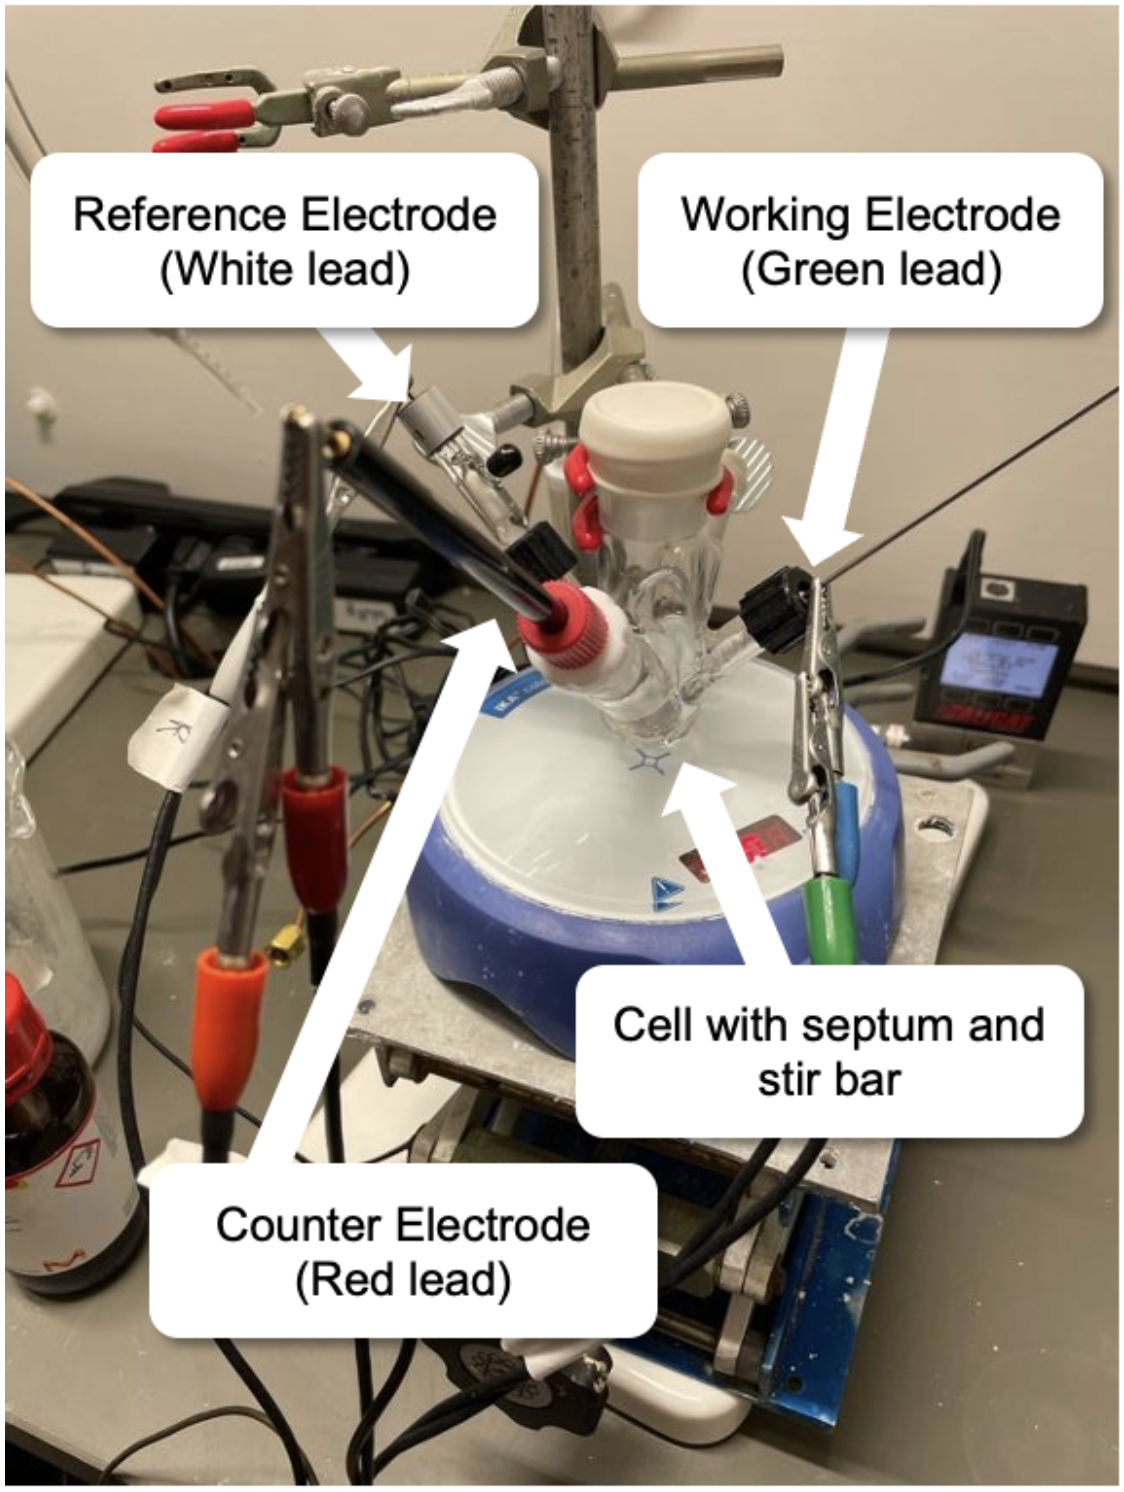
\includegraphics[width=0.4\linewidth]{lab5-setup.png}
    \caption{Experimental setup of the electrochemical cell. The three electrodes (working, reference, and counter) can be seen as well as the container in which the reaction took place. Not immediately pictured is the nitrogen needle used for pre-reaction sparging.}
    \label{fig:setup}
\end{figure}
Ten cycles of a cyclic voltammogram were then taken from \SI{0}{\volt} to \SI{-0.8}{\volt} and back again, and data was recorded vs a \ce{Hg/HgSO4} reference electrode at a scan rate of \SI[per-mode=symbol]{100}{\milli\volt\per\second}. A catalytic wave was observed, and eleven points surrounding its foot were selected for chronoamperometry. These points were evenly spaced in \SI{25}{\milli\volt} intervals. Then, using the computer, the potentiostat was instructed to run the different voltages sequentially from least to greatest. Each voltage was run for \SI{100}{\second} and the diameter of the circular platinum surface was noted to be \SI{2}{\milli\meter} for the purpose of subsequent current density calculations. Throughout the initial (platinum) experiment, continuous stirring should have been applied but was not. However, this did not significantly affect the data, per the TA and lab instructor.\par
The process was repeated for the \ce{Sn} and \ce{Ti} electrodes with stirring enabled, as it should have been. The respective areas of these rectangular electrode was measured with a hand ruler to be $\SI{6}{\milli\meter}\times\SI{8}{\milli\meter}$ and $\SI{7}{\milli\meter}\times\SI{9}{\milli\meter}$. The respective CVs were collected over \SI{0}{\volt} to \SI{-1.8}{\volt} and \SI{0}{\volt} to \SI{-1.6}{\volt}. Due to extreme corrosion and contamination of the solution with tin oxides during the tin experiment, the electrolyte solution was changed between the tin and titanium runs.\par
Lastly, the system was cleaned by safely disposing of the acid electrolyte solution, rinsing everything with milliQ water, and returning all components to their initial spaces.


\subsection*{Results and Discussion}
% Logical stepwise presentation of data and relevant analysis, pointing out important milestones and outcomes (including those reported in figures and tables) along the way.

% The cyclic voltammograms (CV) were taken for each electrode and plotted on an SHE scale, both normalized and unnormalized for the geometric surface area. The CV for unnormalized platinum can be seen in figure 2, the CV for unnormalized titanium can be seen in figure 3, and the CV for unnormalized tin can be seen in figure 4.\par 
% The surface area of each electrode was calculated. The surface area for the platinum electrode was calculated for the area of a circle with a radius of 1 mm. The surface area for the titanium and tin electrodes were calculated by multiplying the width and height which were observed to be 9 mm by 7 mm for titanium and 8 mm by 6 mm for tin. In order to calculate the normalized CVs, the current density was calculated by dividing the current by the surface area. The CV for normalized platinum can be seen in figure 5, the CV for normalized titanium can be seen in figure 6, and the CV for normalized tin can be seen in figure 7. \par
% The onset potential was determined by analyzing the points at the foot of the catalytic wave in the CVs. One point was determined as the onset potential, and ten additional points below and above the onset potential were established to use for the chronoamperogram (CA) data. \par
% The pH of the 0.1 M H2SO4 solution was calculated to be 0.7. From the Pourbaix diagrams given in the lab manual, we can see that the onset potential where H2 and H2O are at equilibrium occurs at roughly 0V for platinum, titanium, and tin for a pH of 0.7. \par
% For platinum, the onset potential was determined from the CV to be -0.05 when adjusted for the SHE scale, which is close to the expected 0V value from the Pourbaix plot. This means that the platinum electrode had an equilibrium between the reduced and oxidized species that was close to what was expected. For titanium, the onset potential was determined from the CV to be -0.66V when adjusted for the SHE scale, which is significantly different from the expected onset potential of 0V from the Pourbaix plot. For tin, the onset potential was determined from the CV to be -0.895V when adjusted for the SHE scale, which is also significantly different from the expected onset potential of 0V. \par
% The curve of the tin plot also had a significantly different shape than expected due to the upward peak on the right side, which might be explained by electrons flowing out of the electrode as the potential passes the equilibrium point and oxygen oxidizing the atoms on the surface of the tin. As the potential becomes negative again, the electrons might have flown back into the electrode and the oxidized atoms could then have been reduced. A similar process likely could have occurred with the titanium electrode to a lower degree.

As described above, the first step was taking cyclic voltammograms for each electrode and replotting the data on an SHE scale, and plotting the $y$-axis as both current and current density.

\begin{figure}[H]
    \centering
    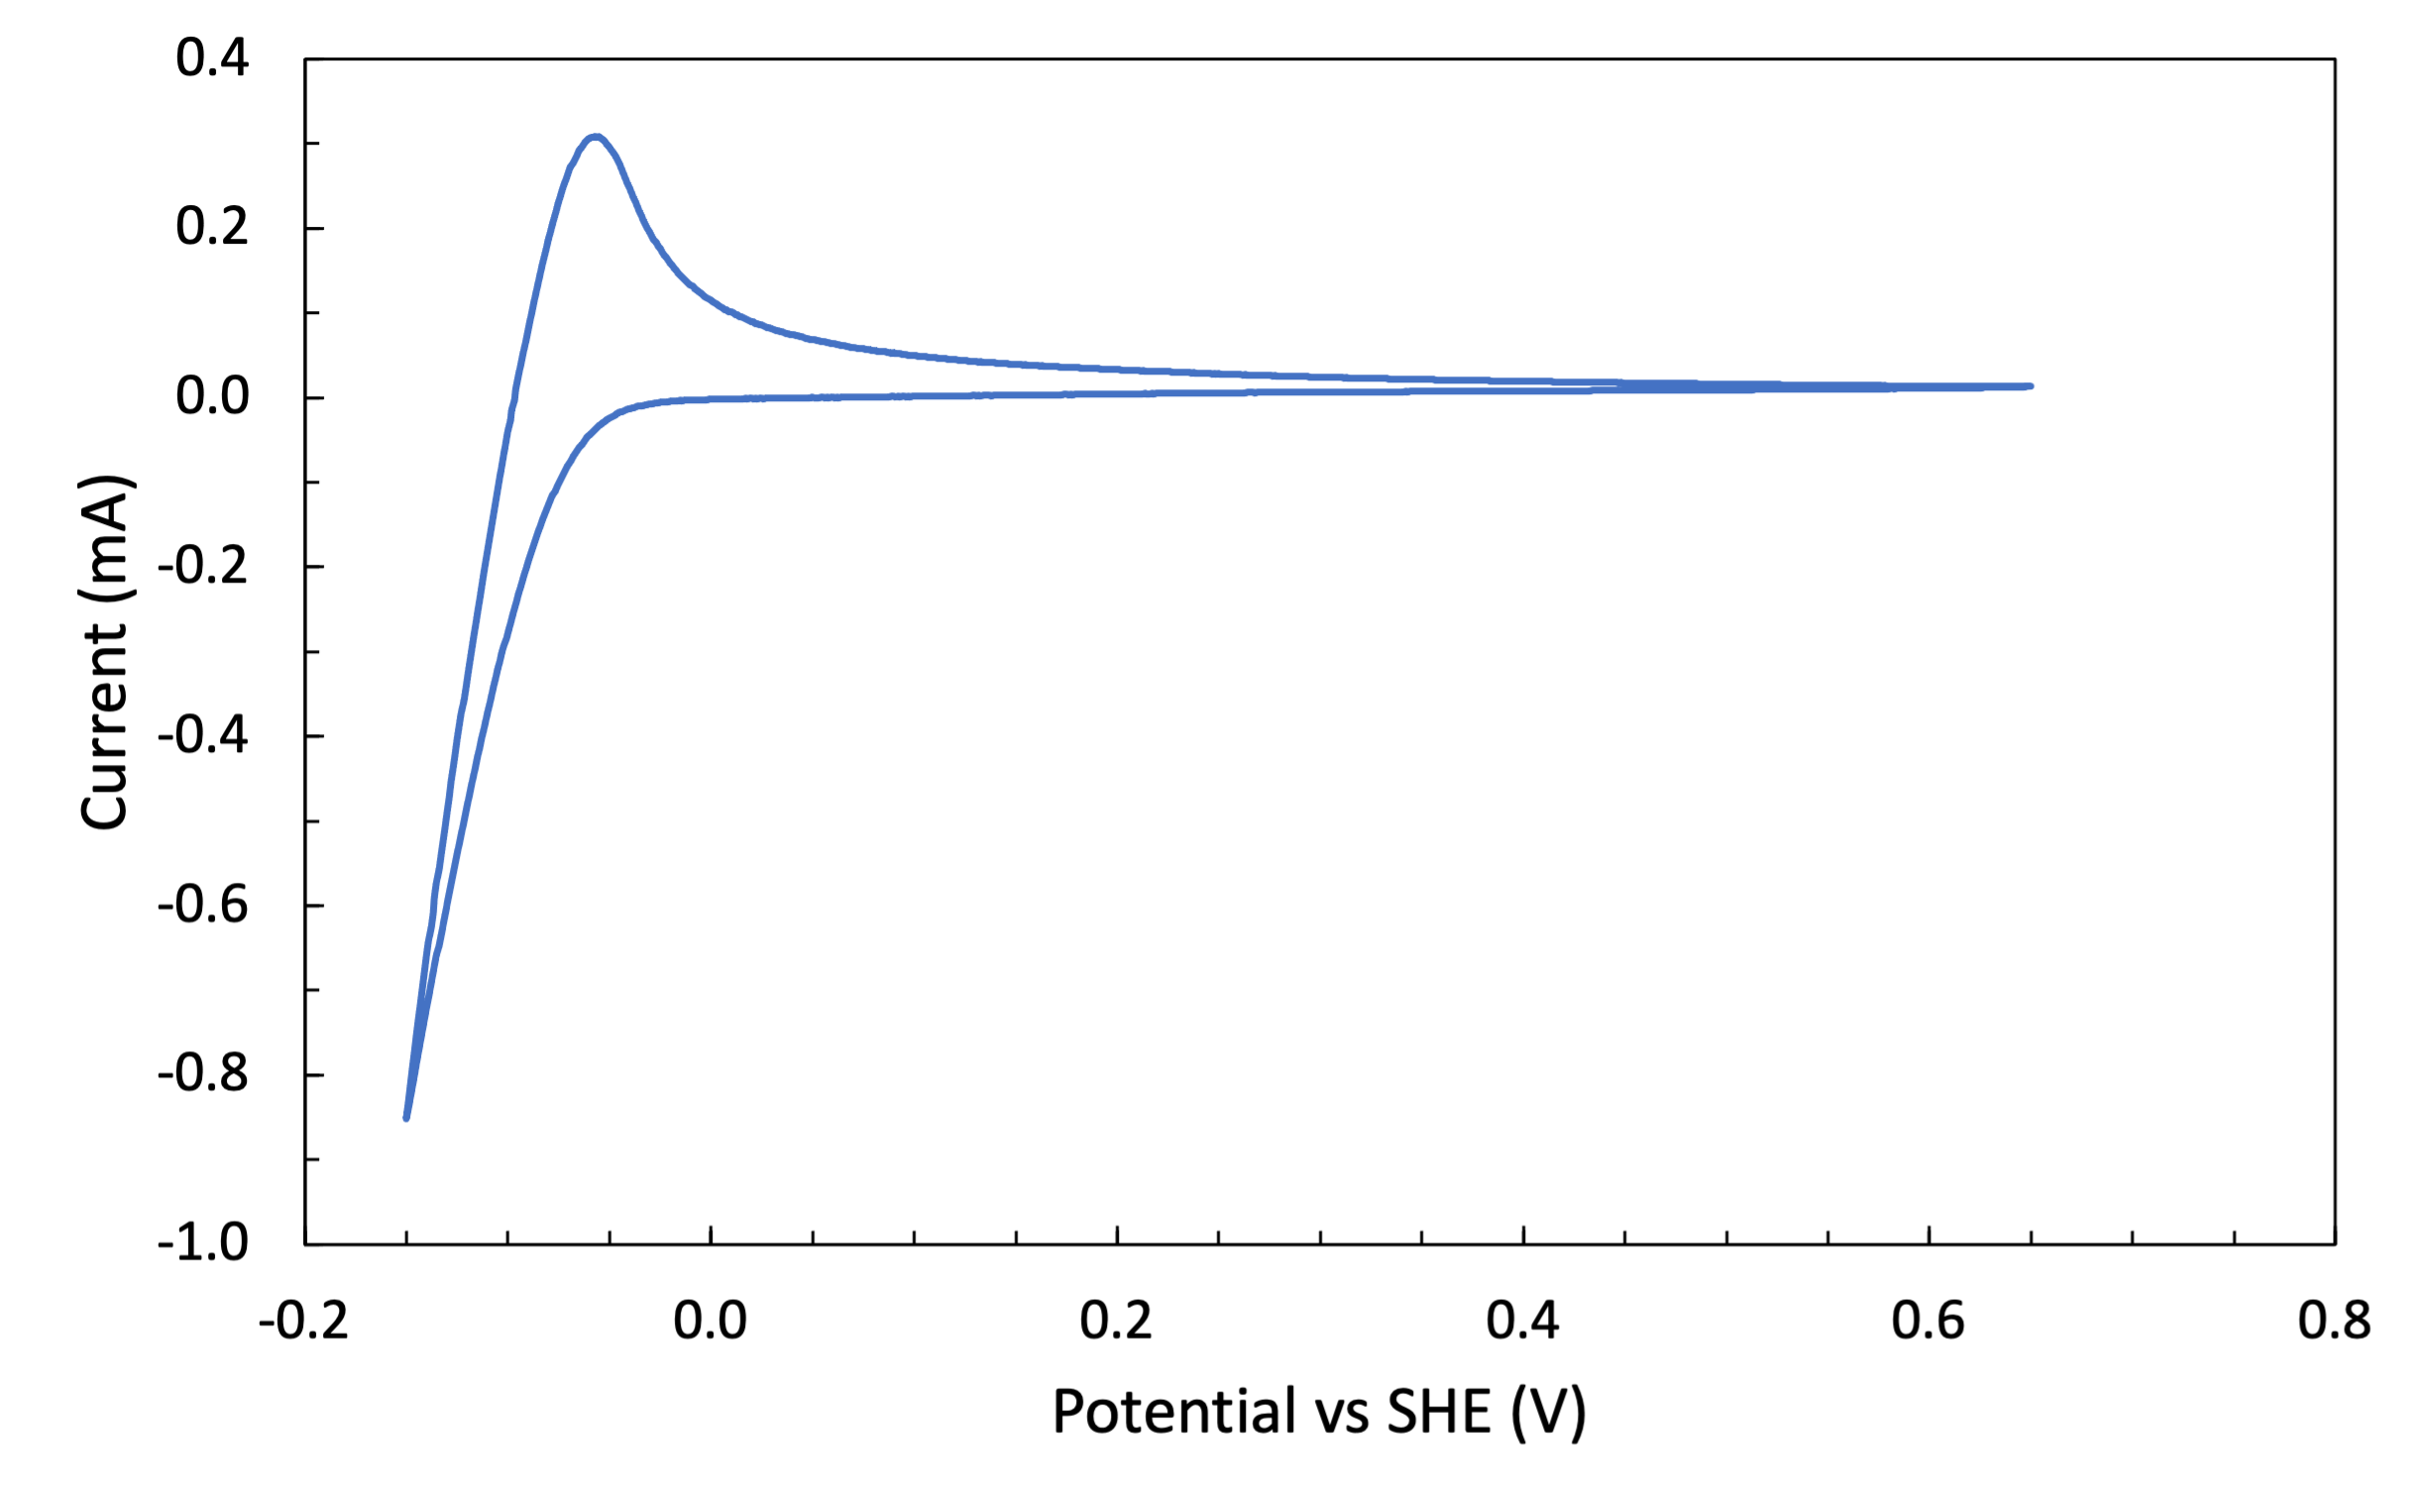
\includegraphics[width=0.95\linewidth]{lab5-CVPtA.png}
    \caption{Extensive cyclic voltammogram exhibiting the HER over a \ce{Pt} electrode in \SI{0.1}{\molar} \ce{H2SO4}. The current (in \si{\milli\ampere}) flowing through the working electrode was measured against the applied potential (in \si{\volt}) as the potential ranged from \SI{0.65}{\volt} to \SI{-0.15}{\volt} vs SHE and back again at a scan rate of \SI[per-mode=symbol]{100}{\milli\volt\per\second}. A middle curve (Curve 4) was selected as representative and plotted in Excel. The HER begins at an overpotential of \SI{0.02}{\volt} vs SHE on the negative scan, and remaining hydrides are oxidized off of the electrode surface on the positive scan resulting in the peak between \SIrange{-0.1}{0}{\volt}.}
    \label{fig:CVPtA}
\end{figure}

\begin{figure}[H]
    \centering
    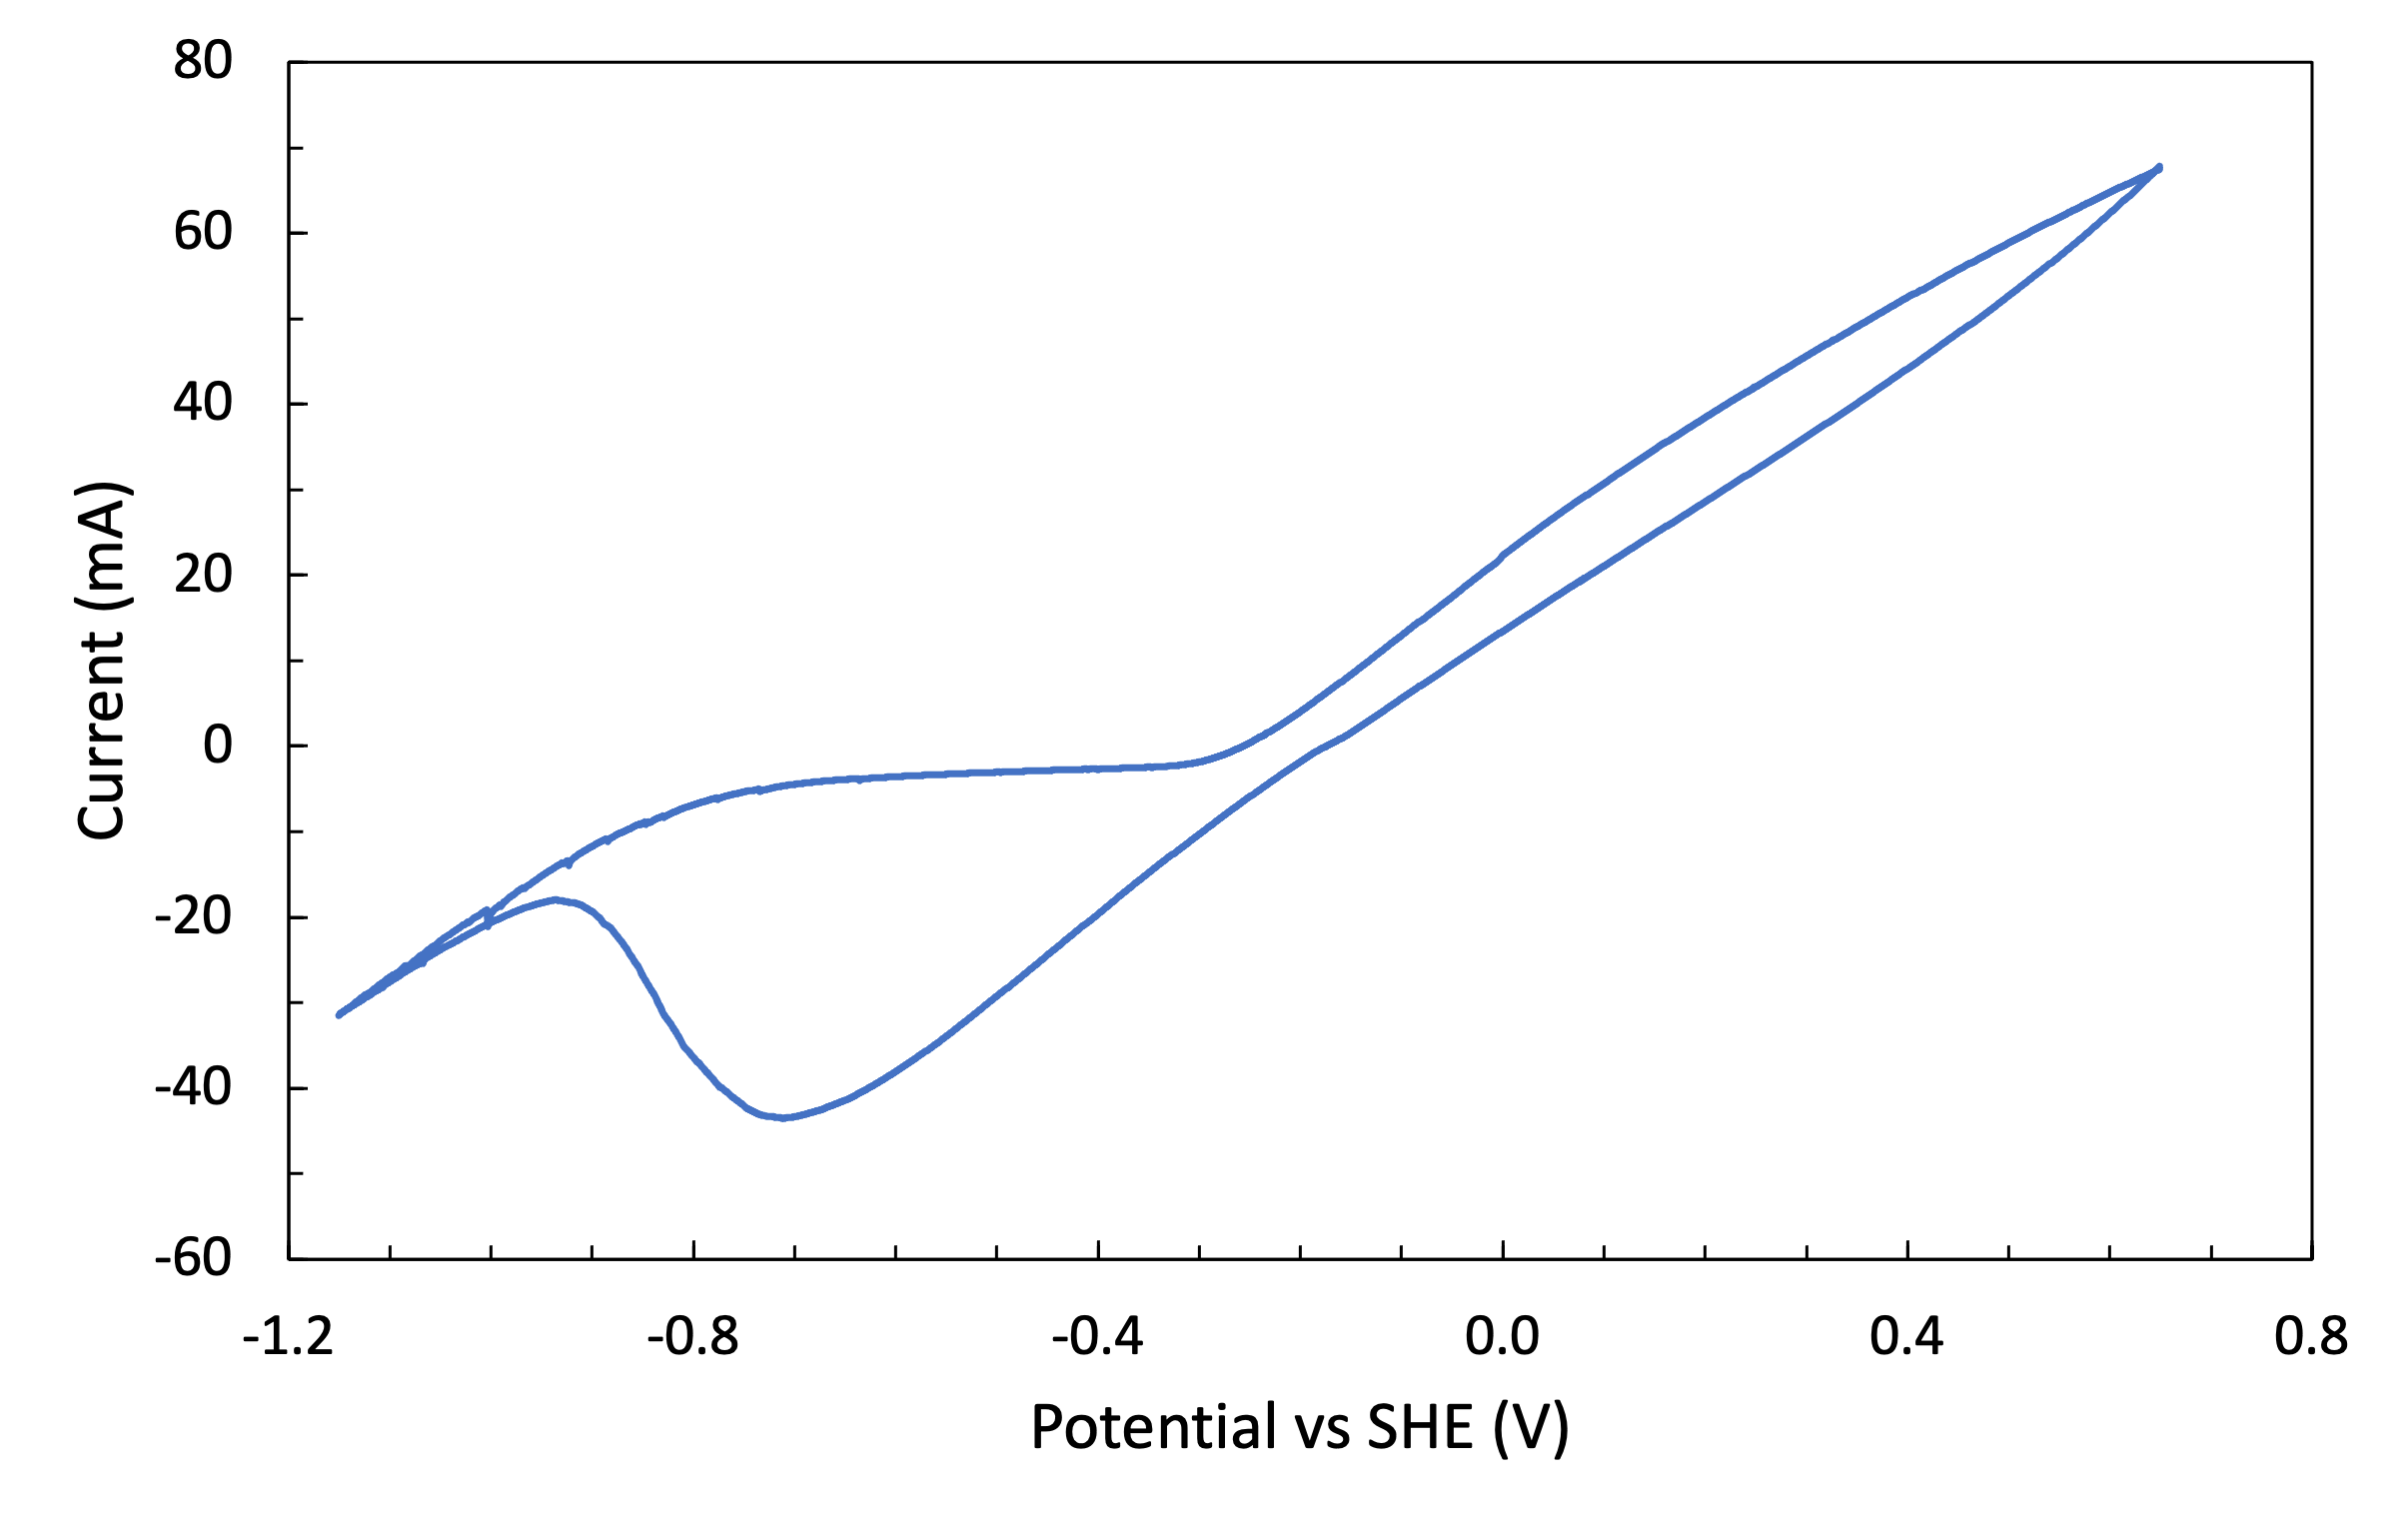
\includegraphics[width=0.95\linewidth]{lab5-CVSnA.png}
    \caption{Extensive cyclic voltammogram exhibiting the HER over a \ce{Sn} electrode in \SI{0.1}{\molar} \ce{H2SO4}. The current (in \si{\milli\ampere}) flowing through the working electrode was measured against the applied potential (in \si{\volt}) as the potential ranged from \SI{0.65}{\volt} to \SI{-1.15}{\volt} vs SHE and back again at a scan rate of \SI[per-mode=symbol]{100}{\milli\volt\per\second}. A middle curve (Curve 4) was selected as representative and plotted in Excel. The HER begins at an overpotential of \SI{0.9}{\volt} vs SHE on the negative scan. No apparent feature correlates with the oxidation of remaining hydrides off of the electrode surface on the positive scan.}
    \label{fig:CVSnA}
\end{figure}

\begin{figure}[H]
    \centering
    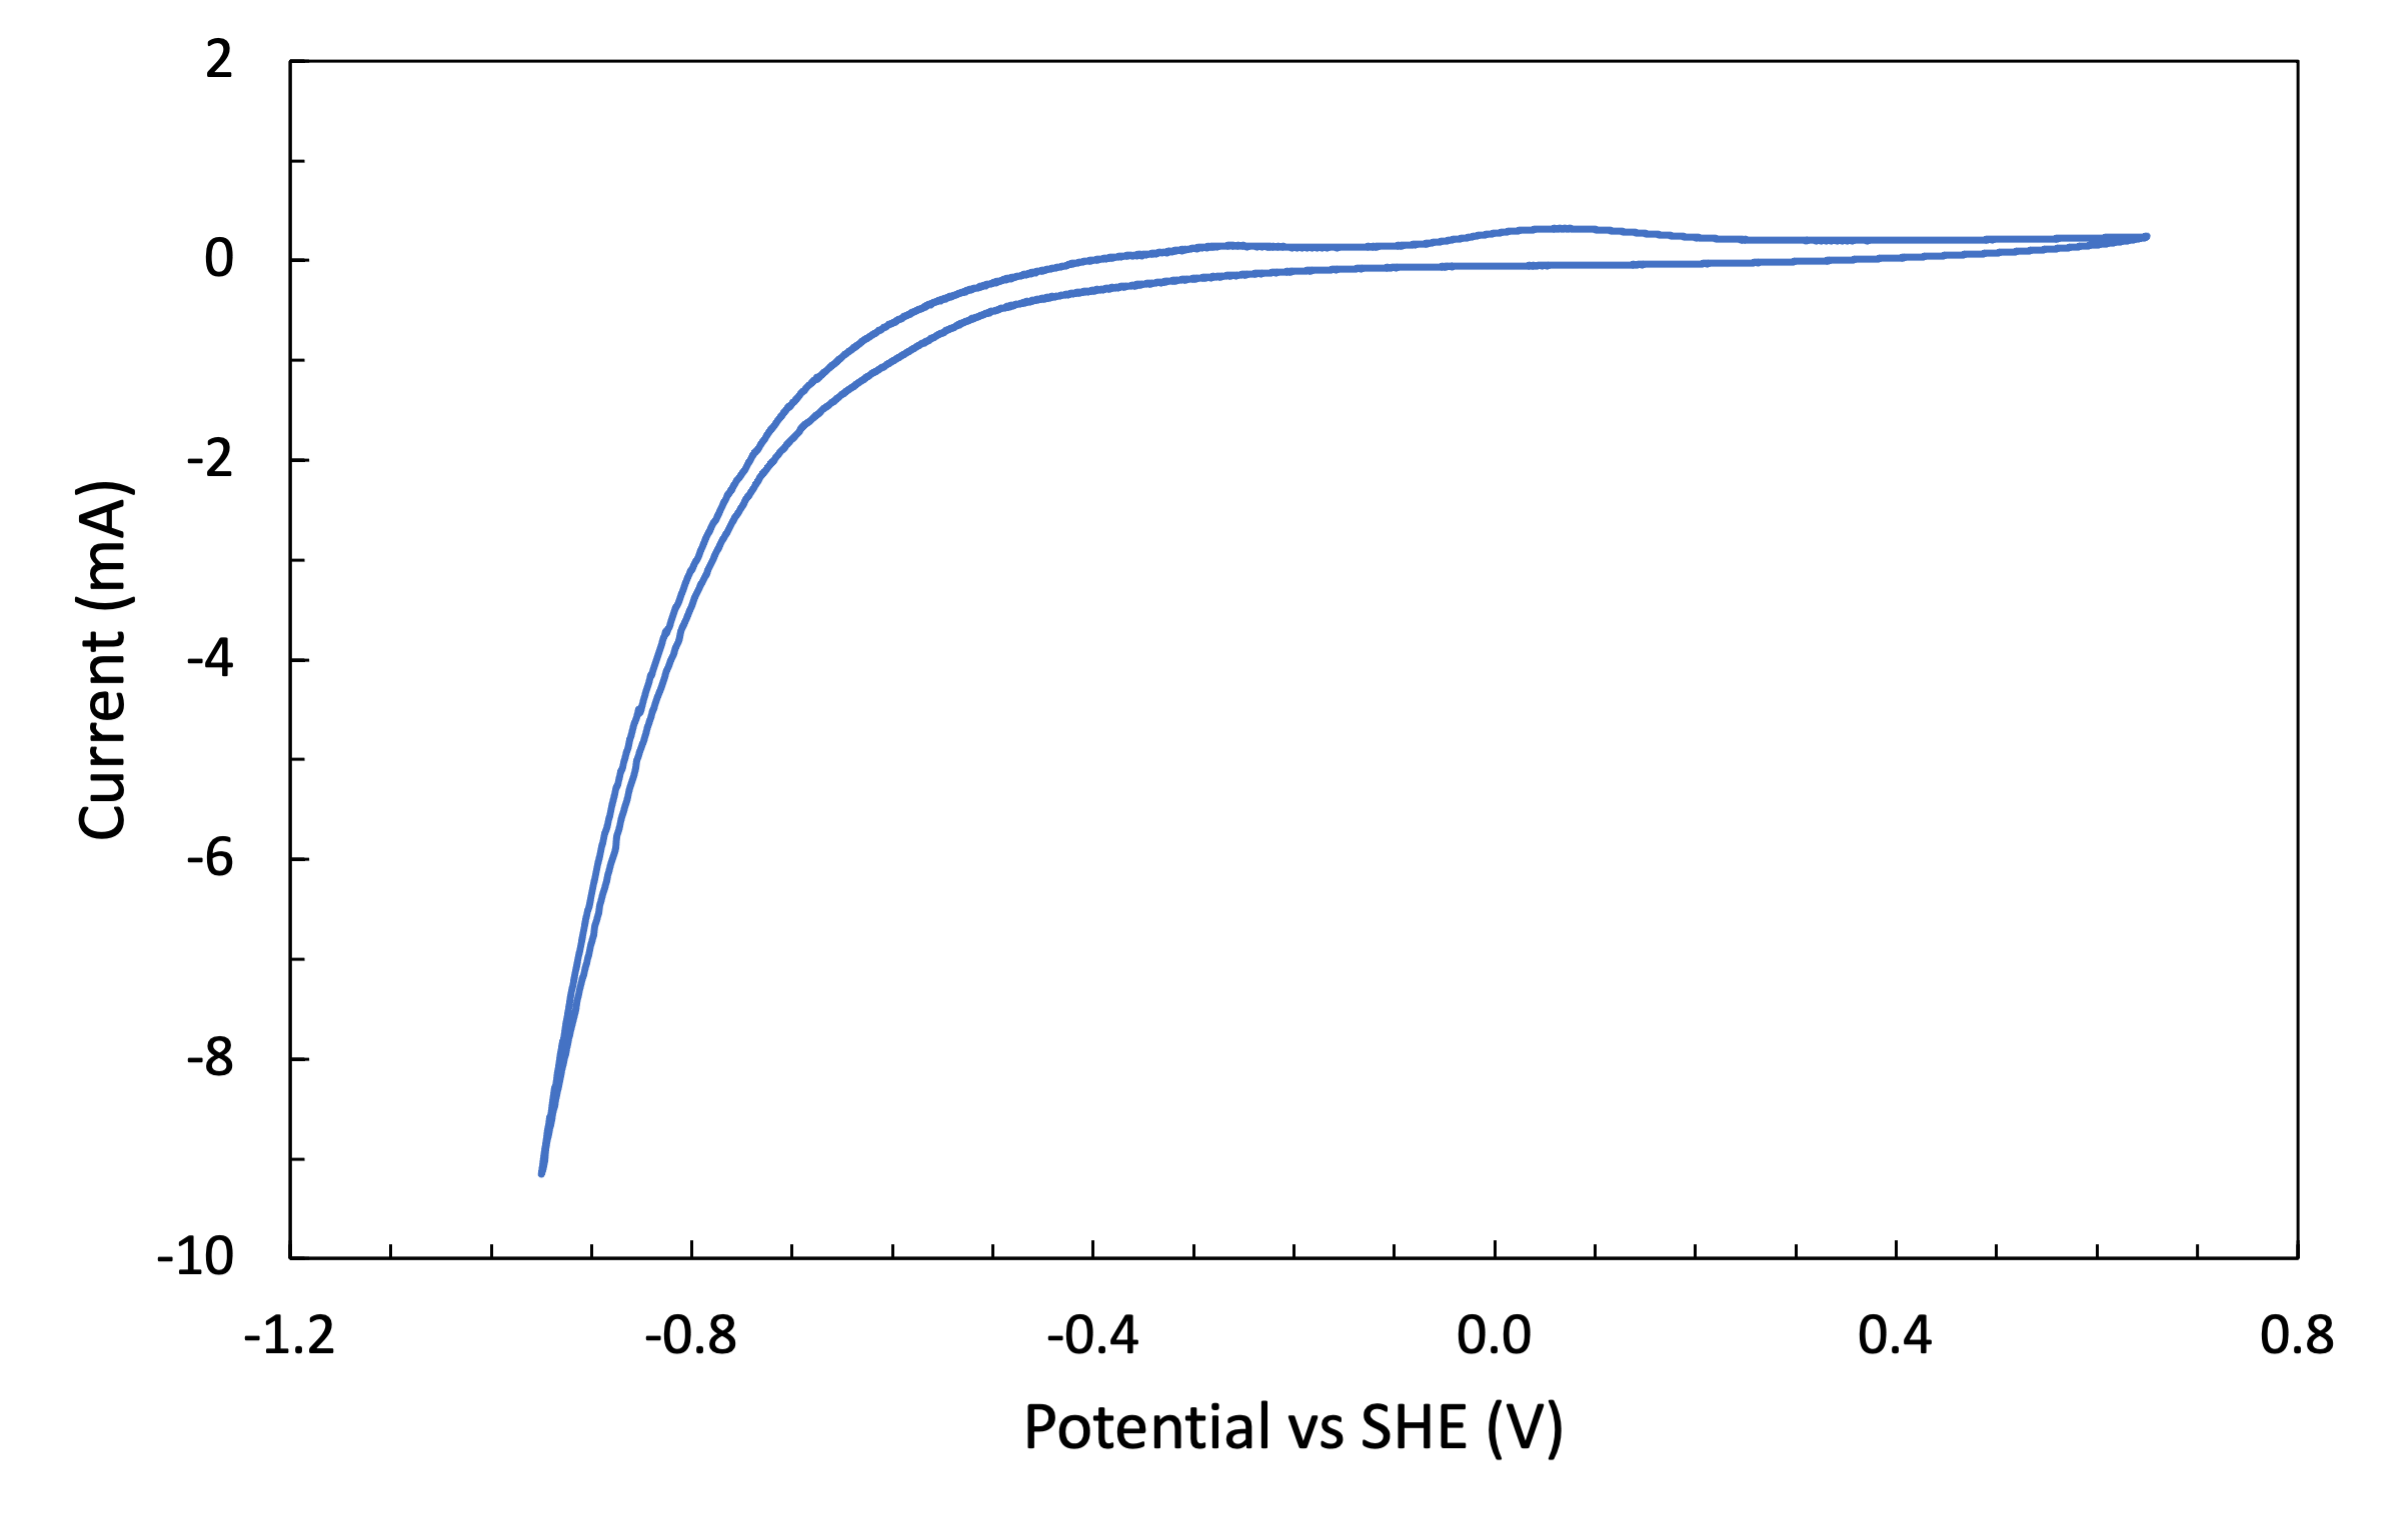
\includegraphics[width=0.95\linewidth]{lab5-CVTiA.png}
    \caption{Extensive cyclic voltammogram exhibiting the HER over a \ce{Ti} electrode in \SI{0.1}{\molar} \ce{H2SO4}. The current (in \si{\milli\ampere}) flowing through the working electrode was measured against the applied potential (in \si{\volt}) as the potential ranged from \SI{0.65}{\volt} to \SI{-0.95}{\volt} vs SHE and back again at a scan rate of \SI[per-mode=symbol]{100}{\milli\volt\per\second}. A middle curve (Curve 4) was selected as representative and plotted in Excel. The HER begins at an overpotential of \SI{0.4}{\volt} vs SHE on the negative scan, and remaining hydrides are oxidized off of the electrode surface on the positive scan resulting in the peak between \SIrange{0}{0.2}{\volt}.}
    \label{fig:CVTiA}
\end{figure}

\begin{figure}[H]
    \centering
    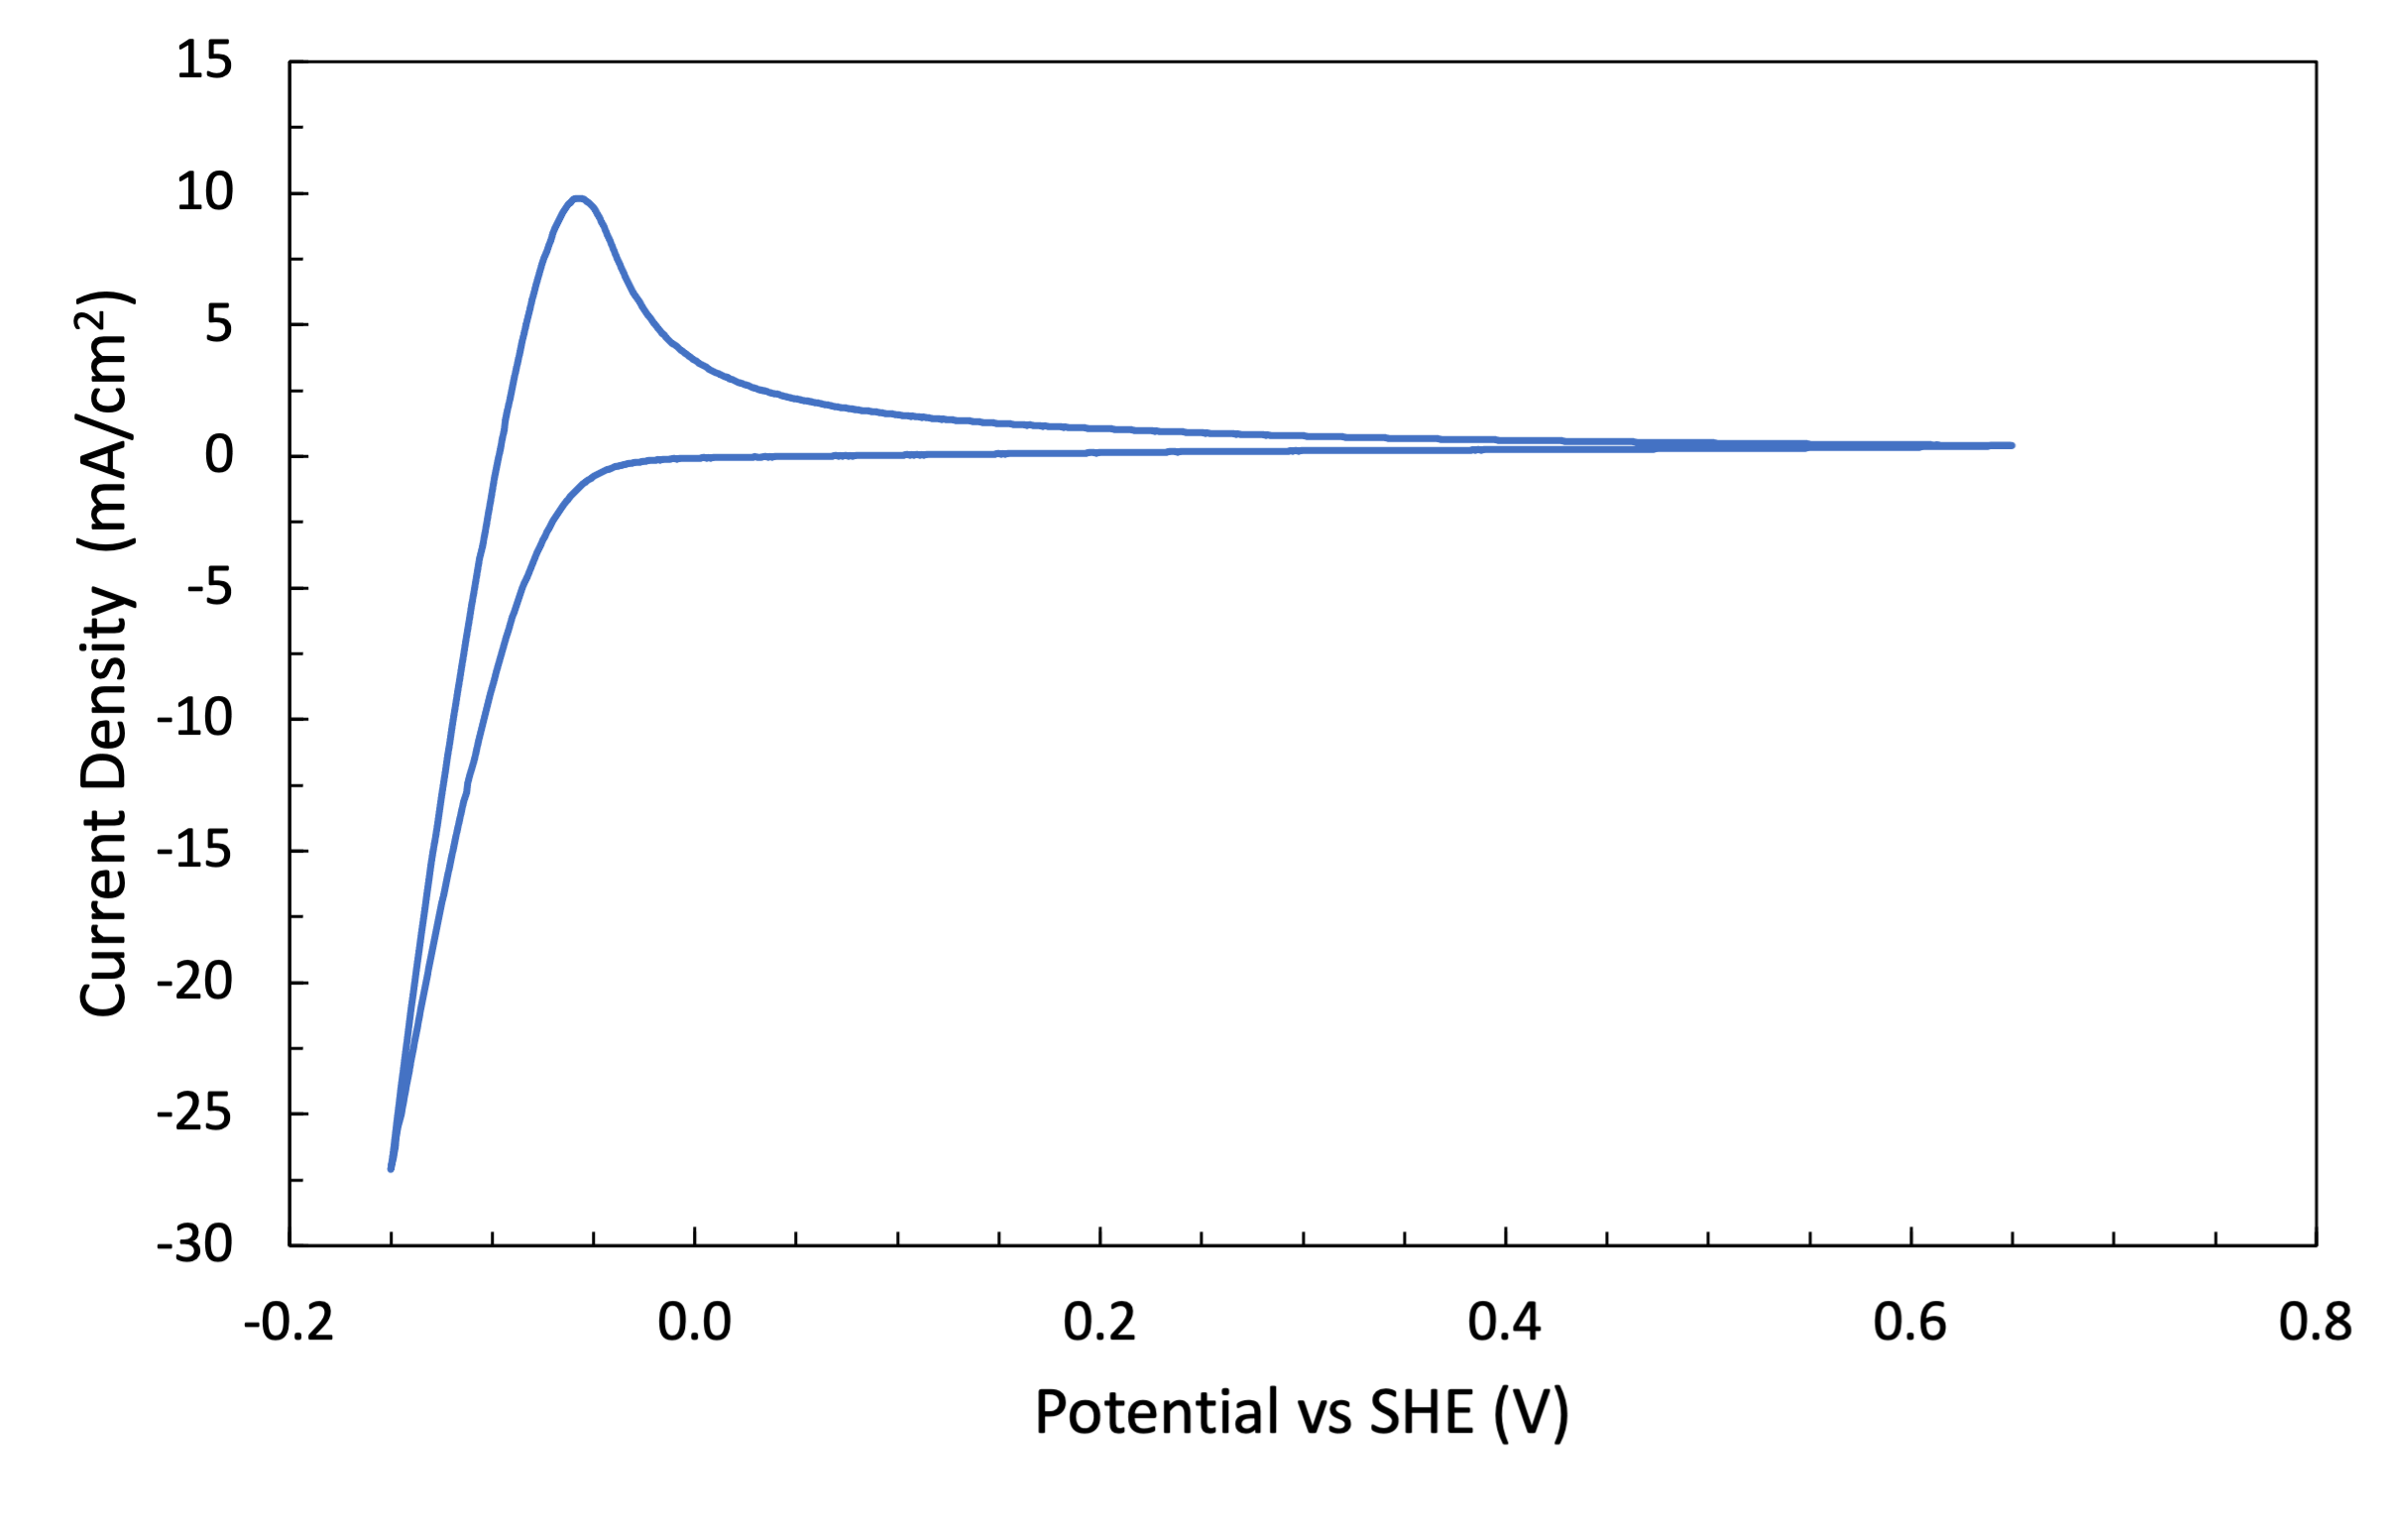
\includegraphics[width=0.95\linewidth]{lab5-CVPtJ.png}
    \caption{Intensive cyclic voltammogram exhibiting the HER over a \ce{Pt} electrode in \SI{0.1}{\molar} \ce{H2SO4}. The current density (in \si[per-mode=symbol]{\milli\ampere\per\centi\meter\squared}) flowing through the working electrode was measured against the applied potential (in \si{\volt}) as the potential ranged from \SI{0.65}{\volt} to \SI{-0.15}{\volt} vs SHE and back again at a scan rate of \SI[per-mode=symbol]{100}{\milli\volt\per\second}. The surface area of the catalyst used in the normalization was \SI{0.0314}{\centi\meter\squared}. A middle curve (Curve 4) was selected as representative and plotted in Excel. The HER begins at an overpotential of \SI{0.02}{\volt} vs SHE on the negative scan, and remaining hydrides are oxidized off of the electrode surface on the positive scan resulting in the peak between \SIrange{-0.1}{0}{\volt}.}
    \label{fig:CVPtJ}
\end{figure}

\begin{figure}[H]
    \centering
    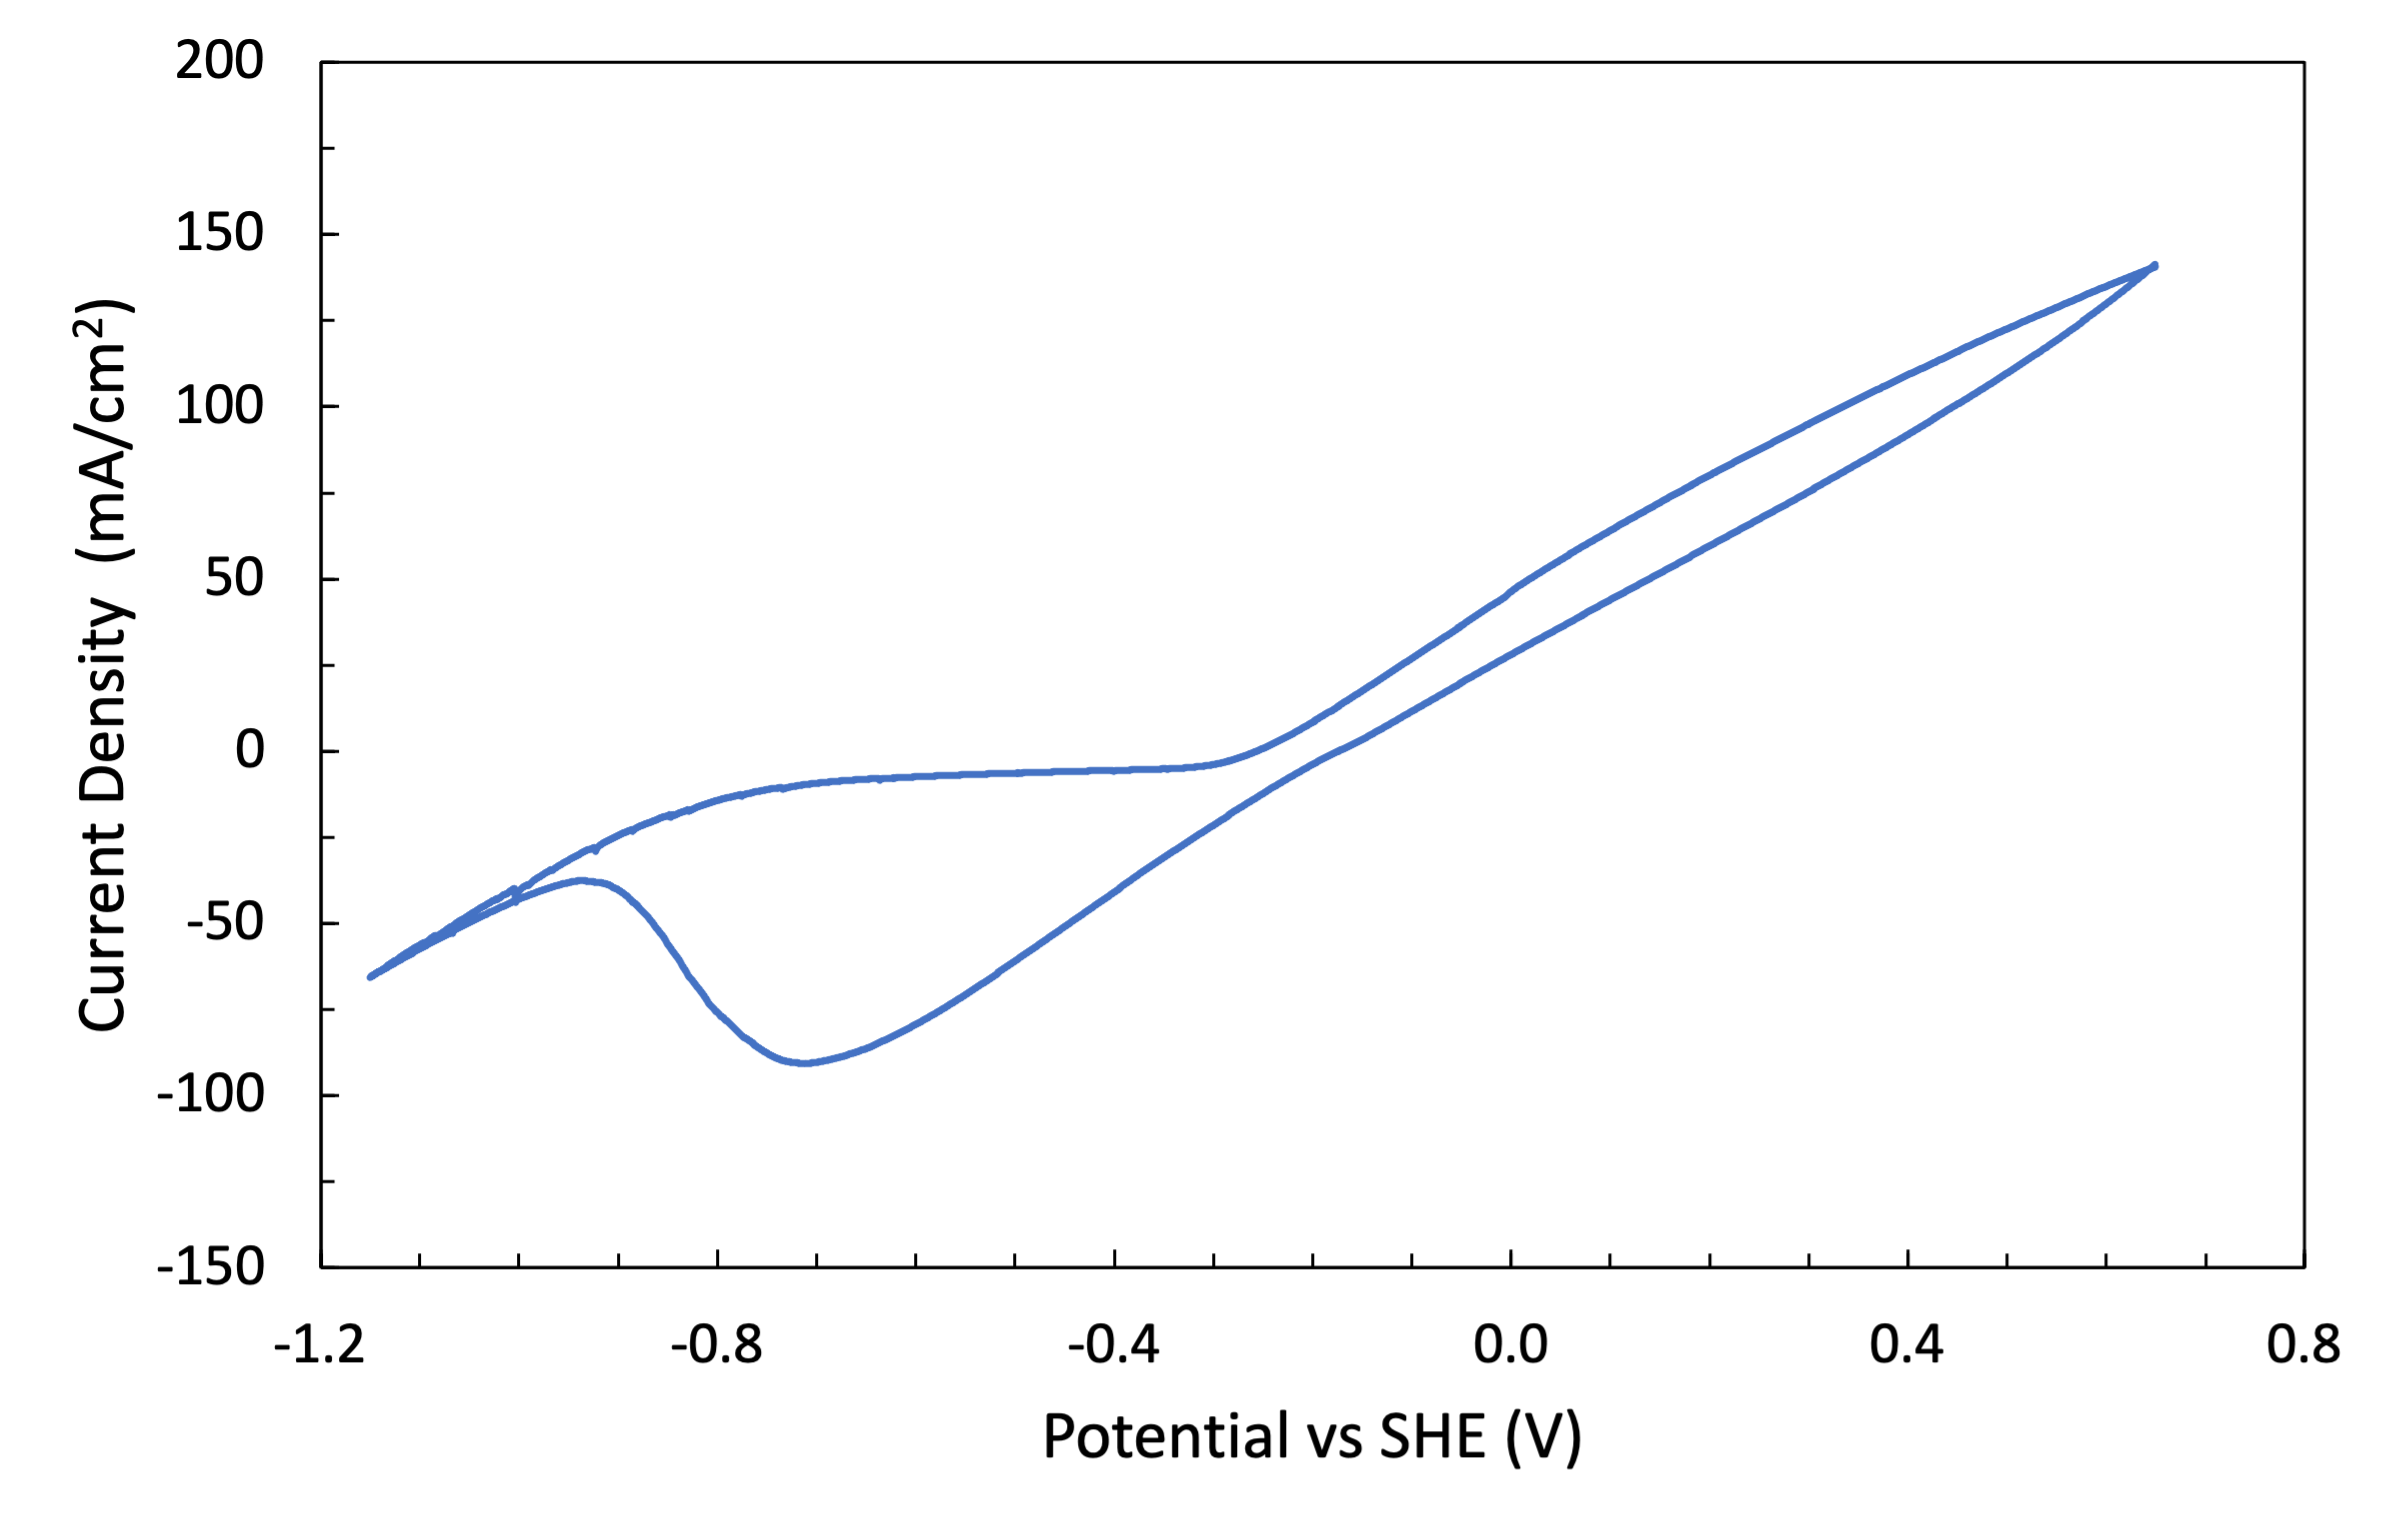
\includegraphics[width=0.95\linewidth]{lab5-CVSnJ.png}
    \caption{Intensive cyclic voltammogram exhibiting the HER over a \ce{Sn} electrode in \SI{0.1}{\molar} \ce{H2SO4}. The current density (in \si[per-mode=symbol]{\milli\ampere\per\centi\meter\squared}) flowing through the working electrode was measured against the applied potential (in \si{\volt}) as the potential ranged from \SI{0.65}{\volt} to \SI{-1.15}{\volt} vs SHE and back again at a scan rate of \SI[per-mode=symbol]{100}{\milli\volt\per\second}. The surface area of the catalyst used in the normalization was \SI{0.48}{\centi\meter\squared}. A middle curve (Curve 4) was selected as representative and plotted in Excel. The HER begins at an overpotential of \SI{0.9}{\volt} vs SHE on the negative scan. No apparent feature correlates with the oxidation of remaining hydrides off of the electrode surface on the positive scan.}
    \label{fig:CVSnJ}
\end{figure}

\begin{figure}[H]
    \centering
    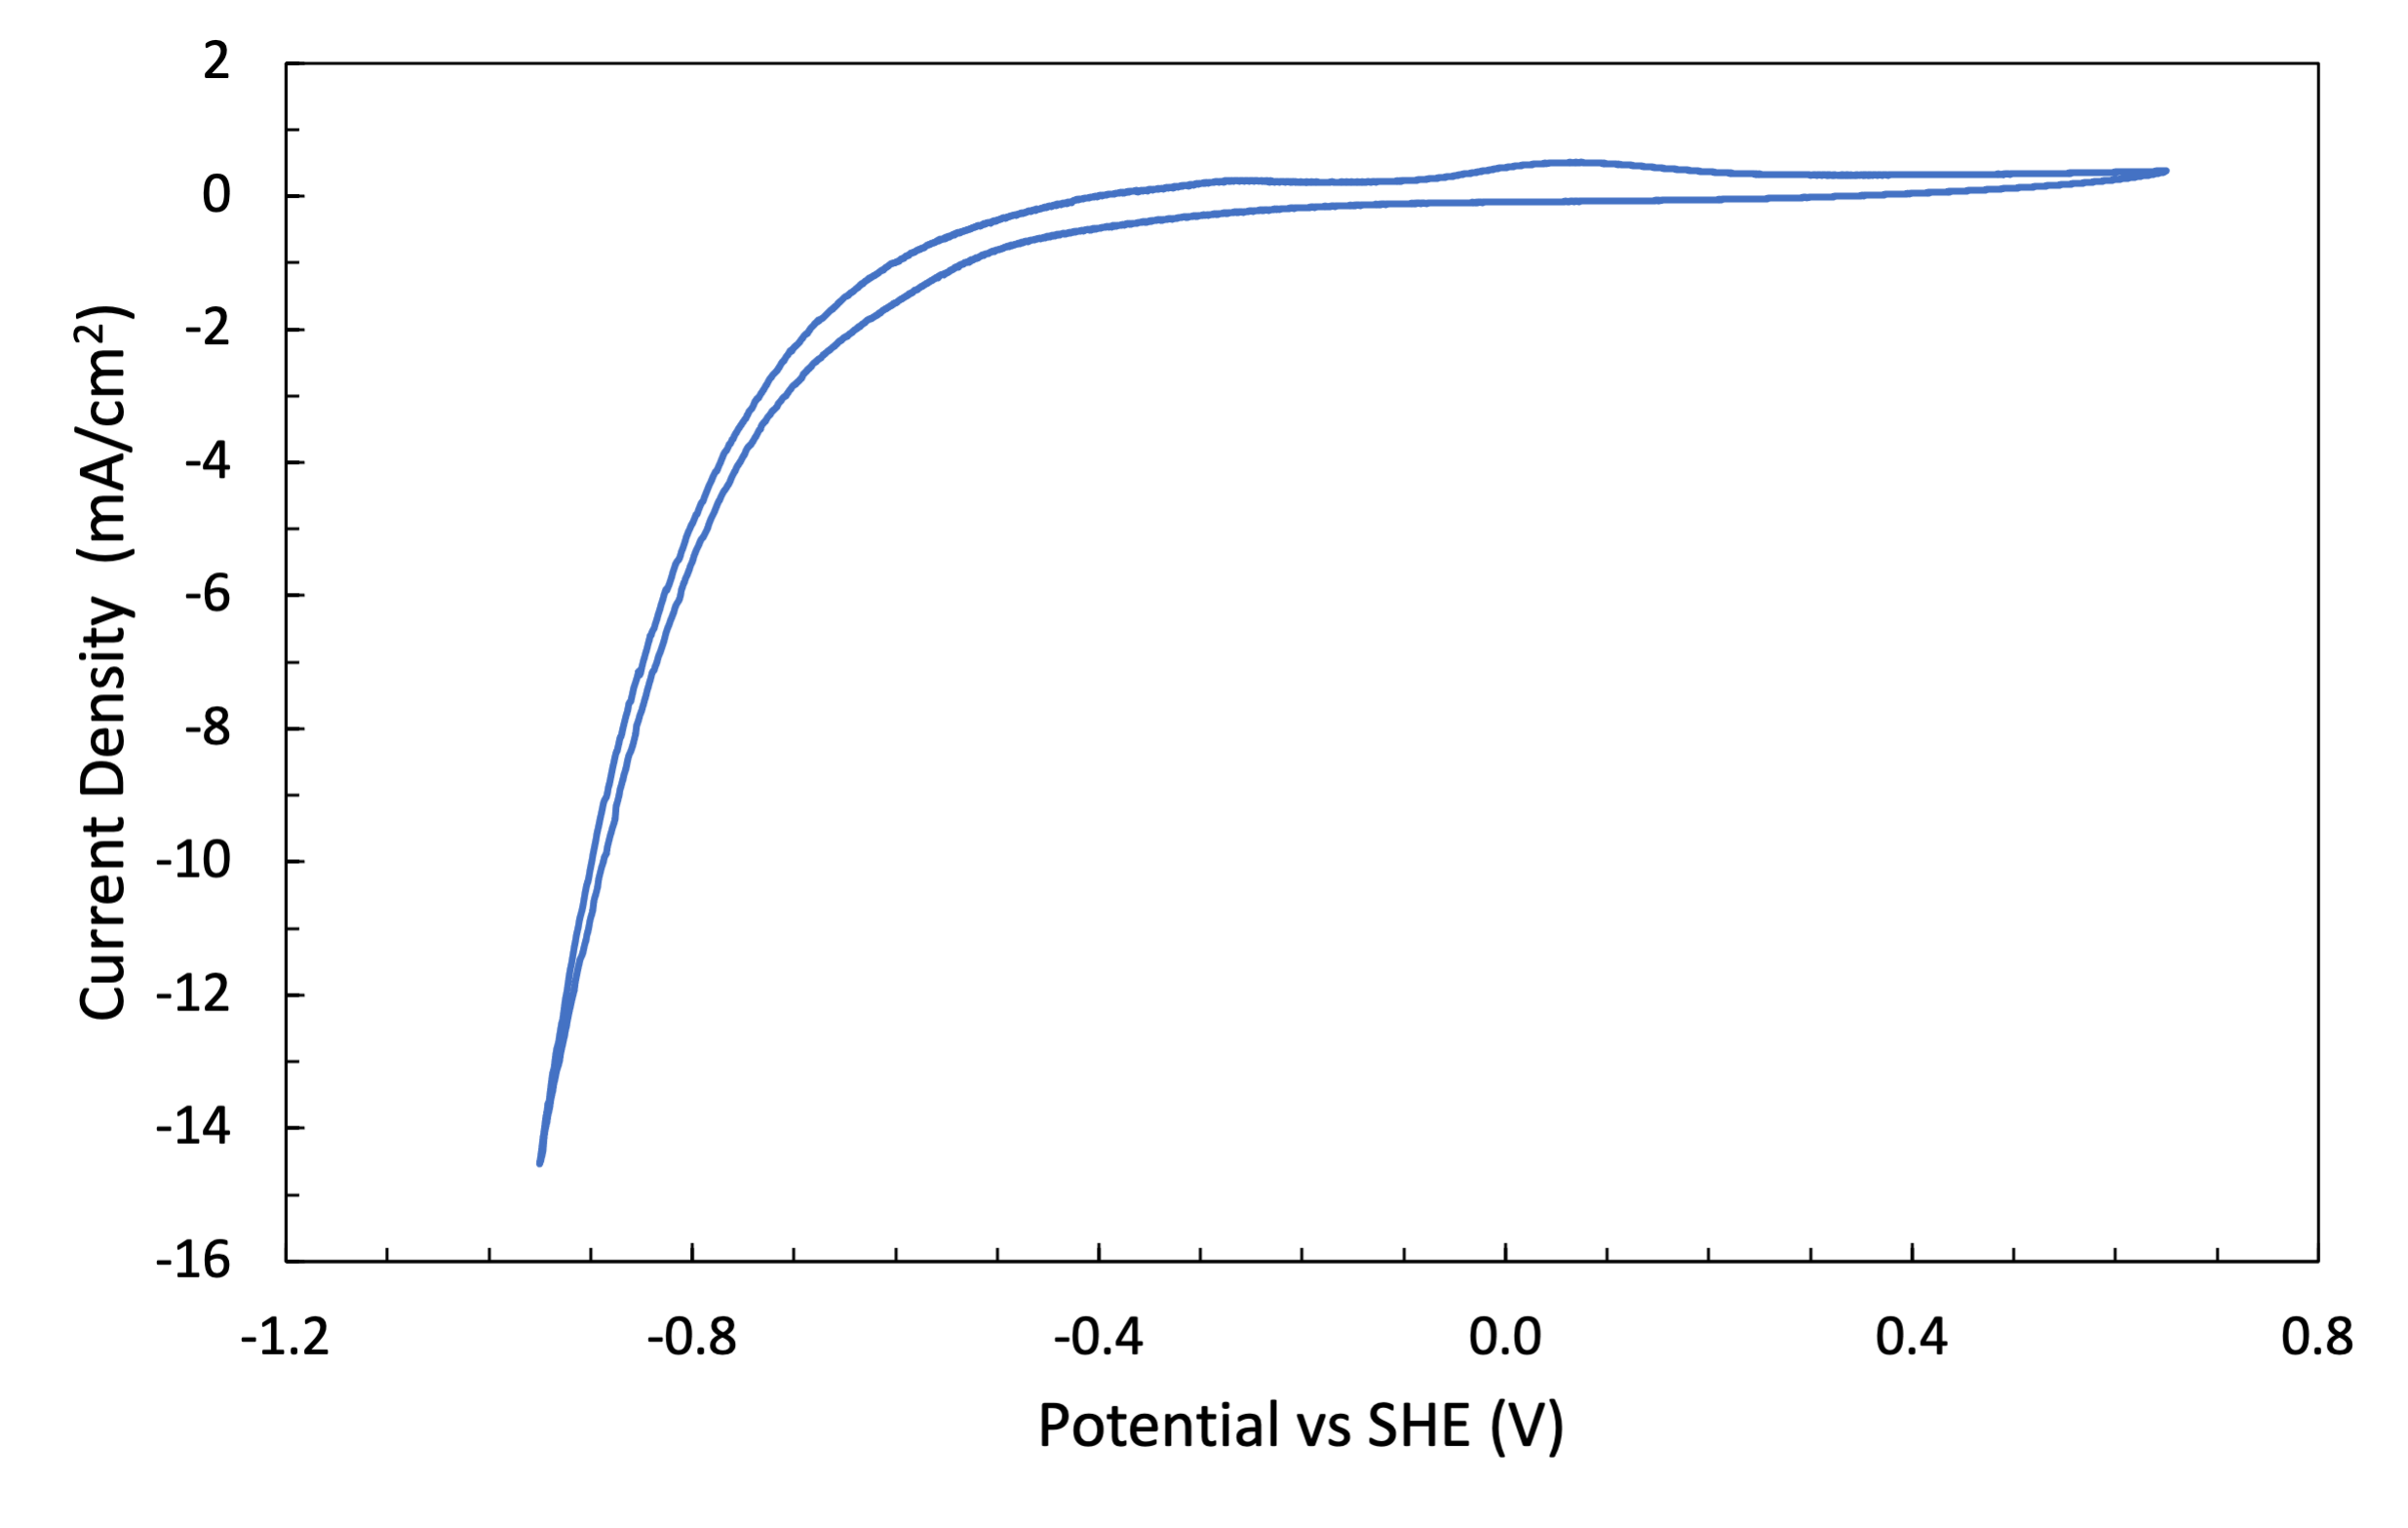
\includegraphics[width=0.95\linewidth]{lab5-CVTiJ.png}
    \caption{Intensive cyclic voltammogram exhibiting the HER over a \ce{Ti} electrode in \SI{0.1}{\molar} \ce{H2SO4}. The current density (in \si[per-mode=symbol]{\milli\ampere\per\centi\meter\squared}) flowing through the working electrode was measured against the applied potential (in \si{\volt}) as the potential ranged from \SI{0.65}{\volt} to \SI{-0.95}{\volt} vs SHE and back again at a scan rate of \SI[per-mode=symbol]{100}{\milli\volt\per\second}. The surface area of the catalyst used in the normalization was \SI{0.63}{\centi\meter\squared}. A middle curve (Curve 4) was selected as representative and plotted in Excel. The HER begins at an overpotential of \SI{0.4}{\volt} vs SHE on the negative scan, and remaining hydrides are oxidized off of the electrode surface on the positive scan resulting in the peak between \SIrange{0}{0.2}{\volt}.}
    \label{fig:CVTiJ}
\end{figure}

% Pt: At $\pH=0.7$, we see that platinum crosses line (a) very close to or at the same potential that it begins catalyzing the HER. \emph{cite atlas?}
% Sn: We observe the formation of \ce{SnO} at potentials above 0 and \ce{SnO2} at potentials above 3'??
% The onset potential in all 3 is around 0.

% Tin was not stable under the reaction conditions and formed a variety of oxides in solution. In addition, the CV process heavily corroded it. 

Since \ce{H2SO4} is a strong diprotic acid, it is safe to assume that it fully dissociates into two equivalents of protons in aqueous solution. Thus,
\begin{equation}
    \pH = -\log[\ce{H3O+}]
    = -\log(0.2)
    \approx 0.7
\end{equation}
Based on the Pourbaix diagrams, all three metals at $\pH=0.7$ cross the HER line (a) at approximately $E=\SI{0}{\volt}$. This agrees well with the foot of the catalytic wave for platinum (see Figures \ref{fig:CVPtA}, \ref{fig:CVPtJ}), but differs significantly for the feet of the catalytic waves for tin and titanium (see Figures \ref{fig:CVSnA}-\ref{fig:CVTiA}, \ref{fig:CVSnJ}-\ref{fig:CVTiJ}). Additionally, the Pourbaix diagram reveals that at higher potentials, the tin electrode forms tin oxides (largely \ce{SnO} and \ce{SnO2}).\supercite{bib:Pourbaix} These likely account for the significant observed corrosion, as high potentials can oxidize the tin atoms at the surface, making them susceptible to nucleophilic attack by the oxygen atoms of water molecules in solution. Note that the extreme corrosion of the tin electrode and presence of additional electrochemical processes (oxide formation) means that the CV measurement and onset potential calculation for the tin electrode is likely not reliable.\par
Thus, the result (supported by both the raw current and current density data) that tin is the most active HER catalyst is likely untrue. Consequently, only platinum and titanium will be considered in this analysis. Both the raw current and the current density data (in particular, the position of the onset potentials) indicate that platinum is more active.\par
Although it didn't matter in this case, note that the plot of current \emph{density} vs. voltage is a more accurate reflection of the intrinsic activity of each electrode material than the plot of raw current vs. voltage. This is because naturally a larger quantity of material will transfer more electrons by virtue of sheer active site size. However, this is an \emph{extensive} property, and normalizing for the surface area allows for the comparison of \emph{intensive} properties of the material. These are actually characteristic and thus of greater interest and validity. See the Introduction for more detail on extensive and intensive properties.\par
Additionally, while normalization by the geometric surface area is good, alternate methods of normalization may yield even better data. One example is the determination of the \emph{electrochemical active} surface area.\supercite{bib:EASA} On an atomic scale, not all sites on the surface of the electrode will be equally conducive to electrochemistry, so directly measuring which ones are can give a more accurate representation of current density.\par
Returning to the earlier idea of onset potential, recall that the onset potential was determined by analyzing points at the foot of the catalytic waves. This region of high change in current makes it naturally suited to collecting CA data. Thus, chronoamperograms were collected at the onset potential, at five higher potentials, and at five lower potentials. The potentials were all equally spaced \SI{25}{\milli\volt} apart. This allowed for the construction of the Tafel plots below. For the exact method of construction, see the relevant Excel files.

\begin{figure}[H]
    \centering
    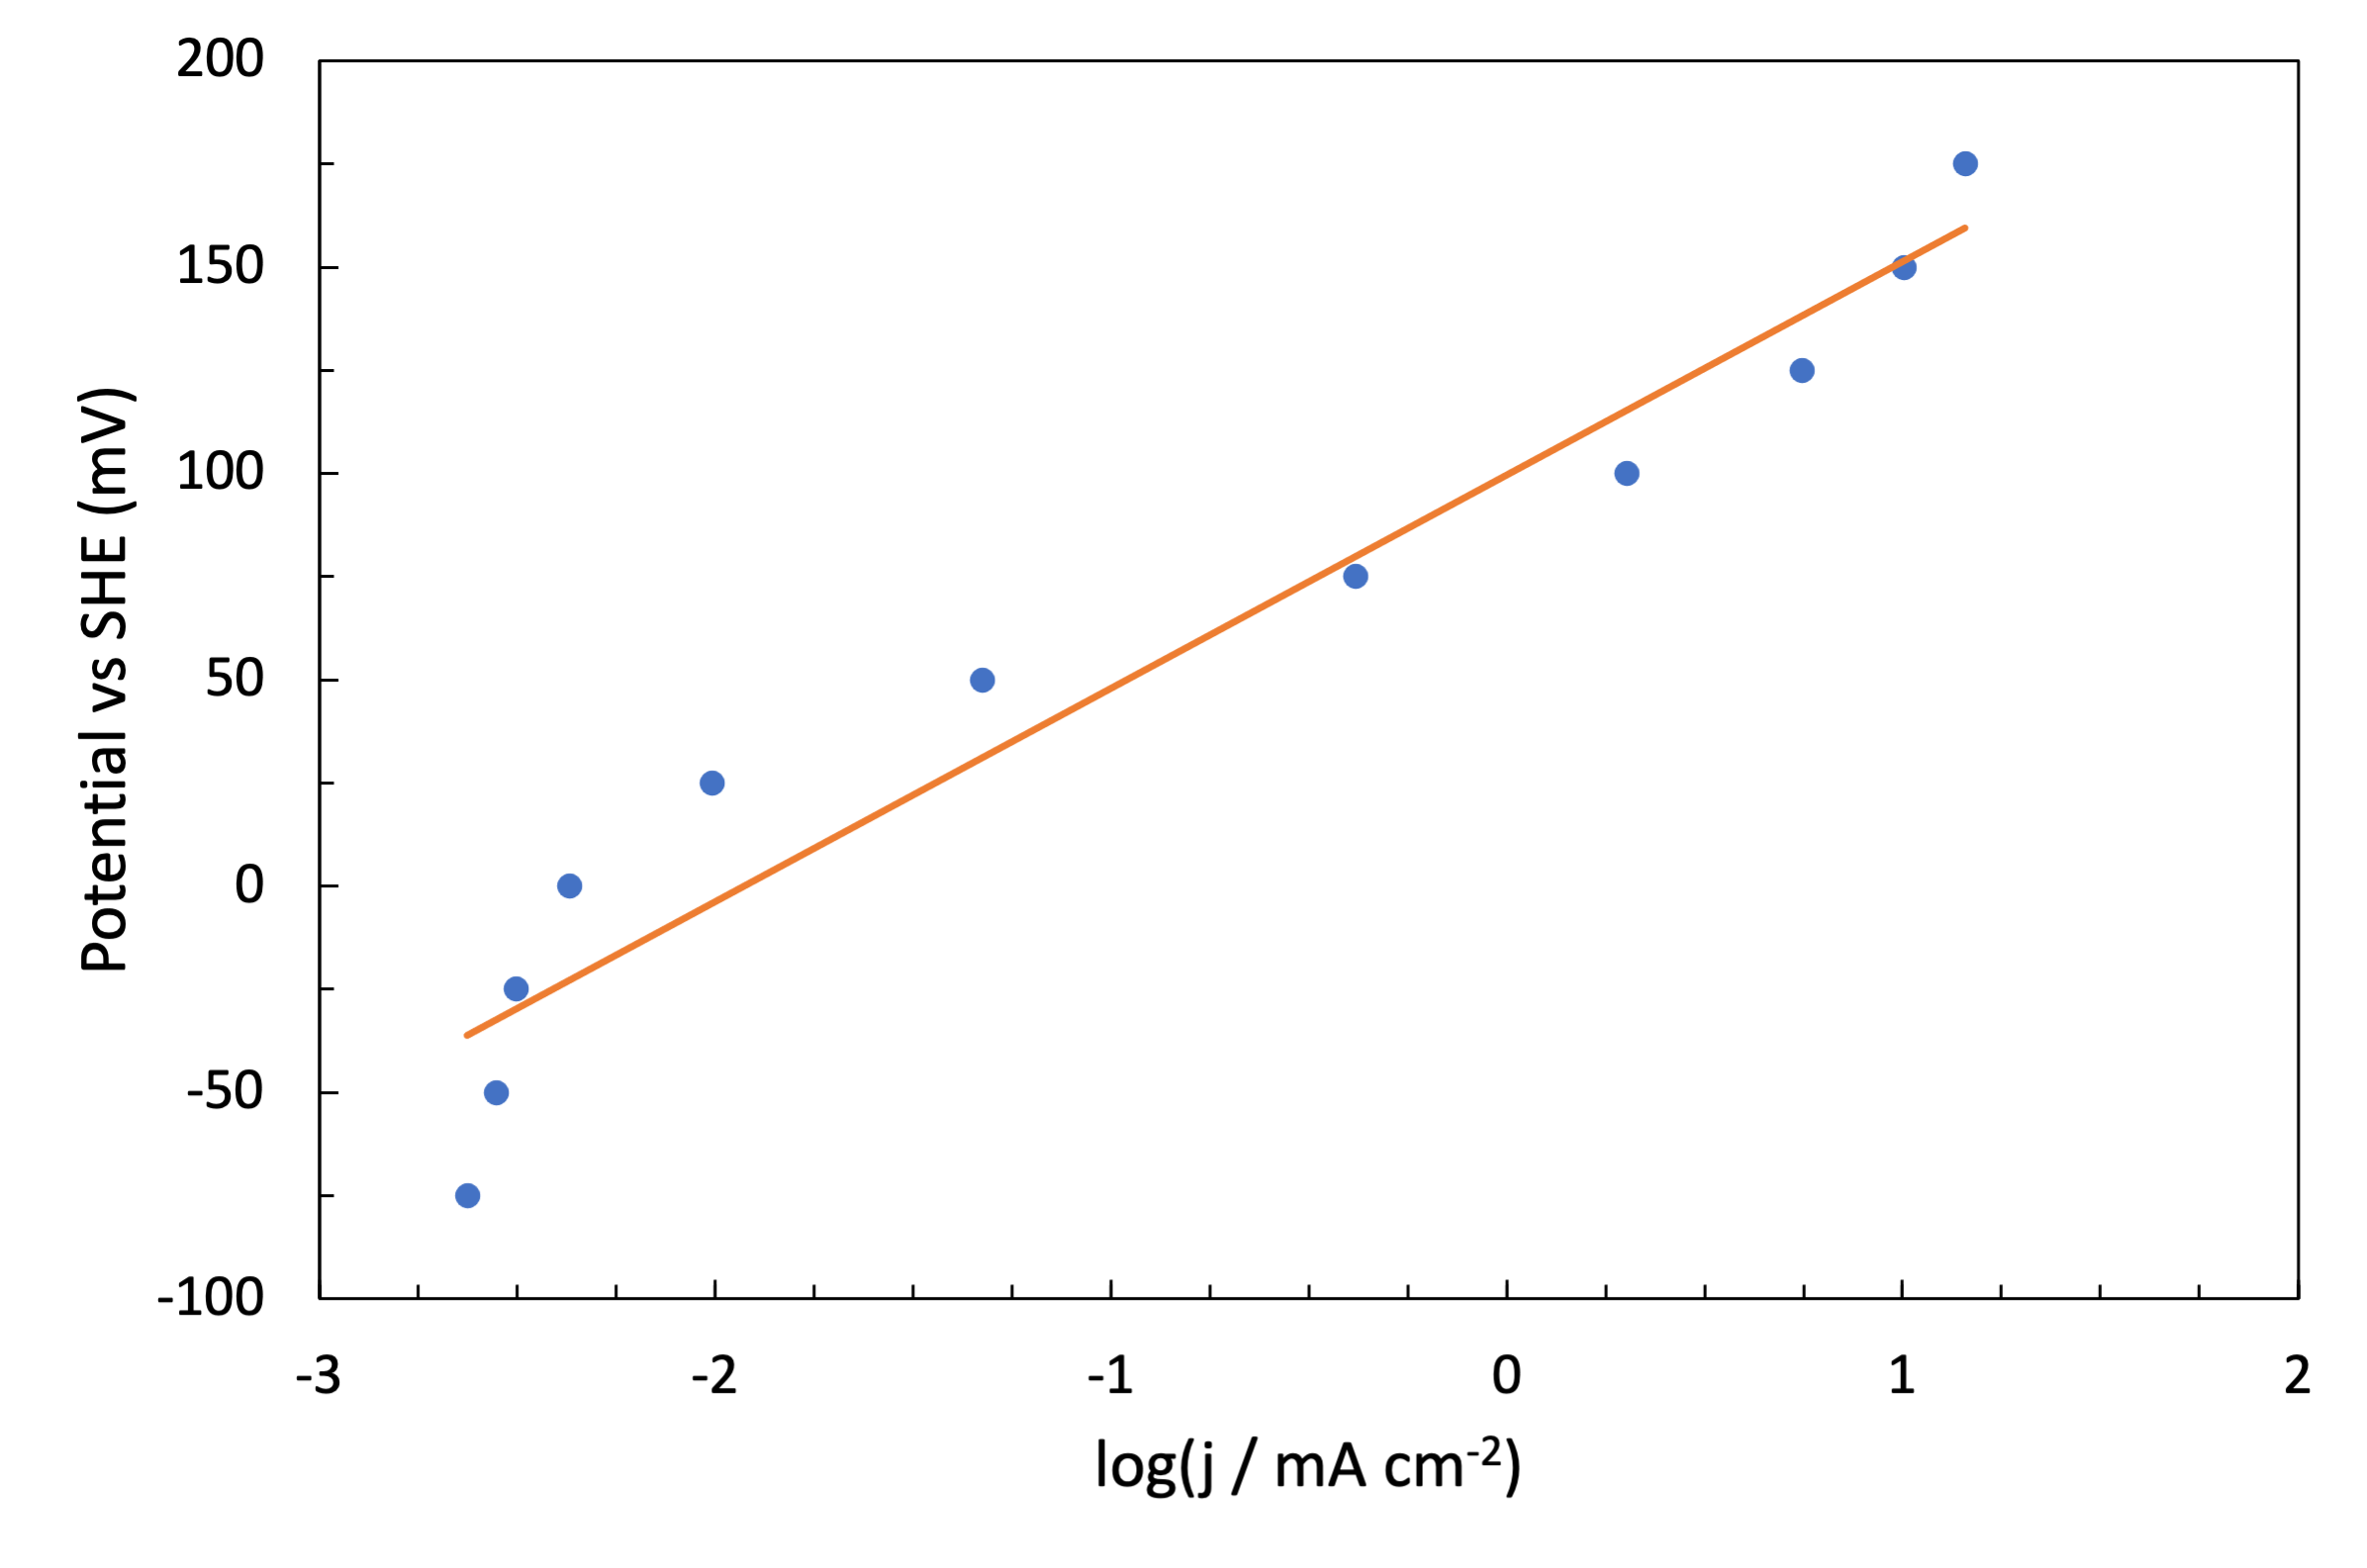
\includegraphics[width=0.95\linewidth]{lab5-CAPt.png}
    \caption{Tafel plot for the HER over a \ce{Pt} electrode in \SI{0.1}{\molar} \ce{H2SO4}. The potentials (in \si{\volt}) were selected on the basis of preceding cyclic voltammetry experiments to surround the foot of the catalytic wave in \SI{25}{\milli\volt} intervals. The logarithmic current densities were calculated from the average current measured at each potential in the last \SI{30}{\second} of a \SI{100}{\second} cyclic amperometry experiment conducted at a given potential, and normalized using the platinum electrode surface area of \SI{0.0314}{\centi\meter\squared}. Data analysis and linear regression was performed in Excel using the Solver function. A positive Tafel slope is observed: $m=\SI{48}{\milli\volt/dec}$ and $b=\SI{101}{\milli\volt}$ for a fit to $\eta=m\cdot\log(j)+b$.}
    \label{fig:CAPt}
\end{figure}

\begin{figure}[H]
    \centering
    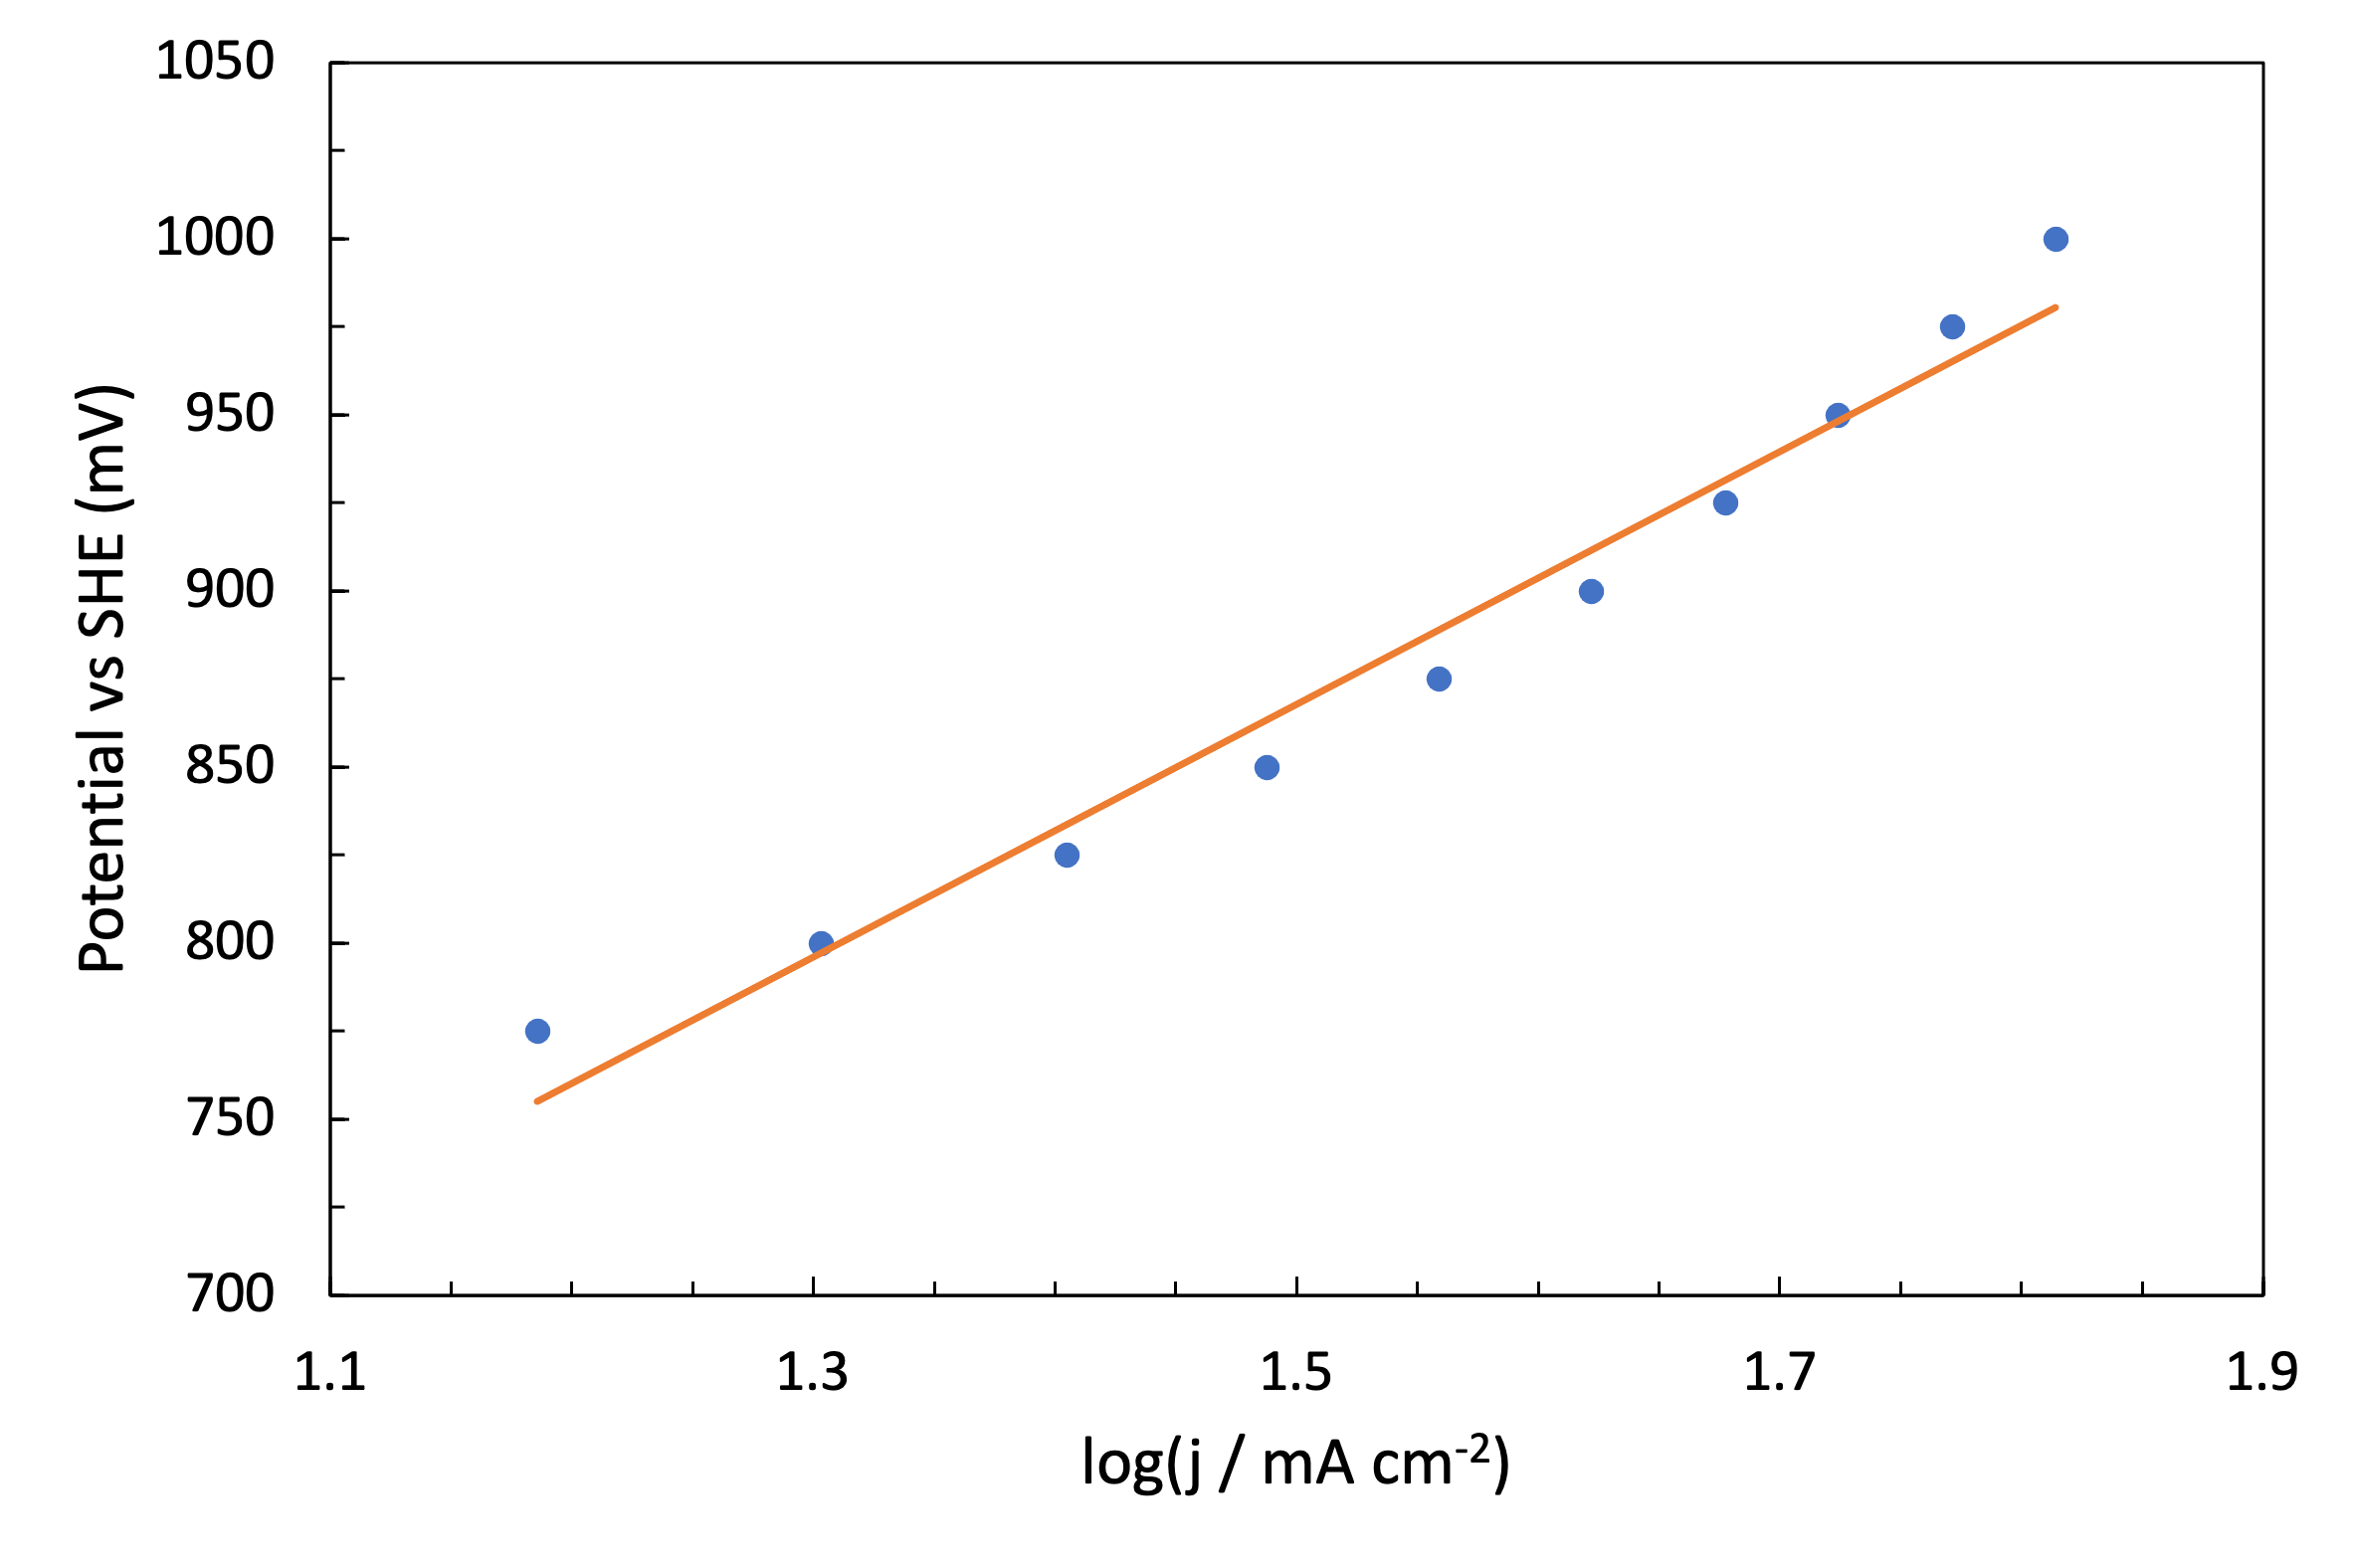
\includegraphics[width=0.95\linewidth]{lab5-CASn.png}
    \caption{Tafel plot for the HER over a \ce{Sn} electrode in \SI{0.1}{\molar} \ce{H2SO4}. The potentials (in \si{\volt}) were selected on the basis of preceding cyclic voltammetry experiments to surround the foot of the catalytic wave in \SI{25}{\milli\volt} intervals. The logarithmic current densities were calculated from the average current measured at each potential in the last \SI{30}{\second} of a \SI{100}{\second} cyclic amperometry experiment conducted at a given potential, and normalized using the tin electrode surface area of \SI{0.48}{\centi\meter\squared}. Data analysis and linear regression was performed in Excel using the Solver function. A positive Tafel slope is observed: $m=\SI{359}{\milli\volt/dec}$ and $b=\SI{330}{\milli\volt}$ for a fit to $\eta=m\cdot\log(j)+b$.}
    \label{fig:CASn}
\end{figure}

\begin{figure}[H]
    \centering
    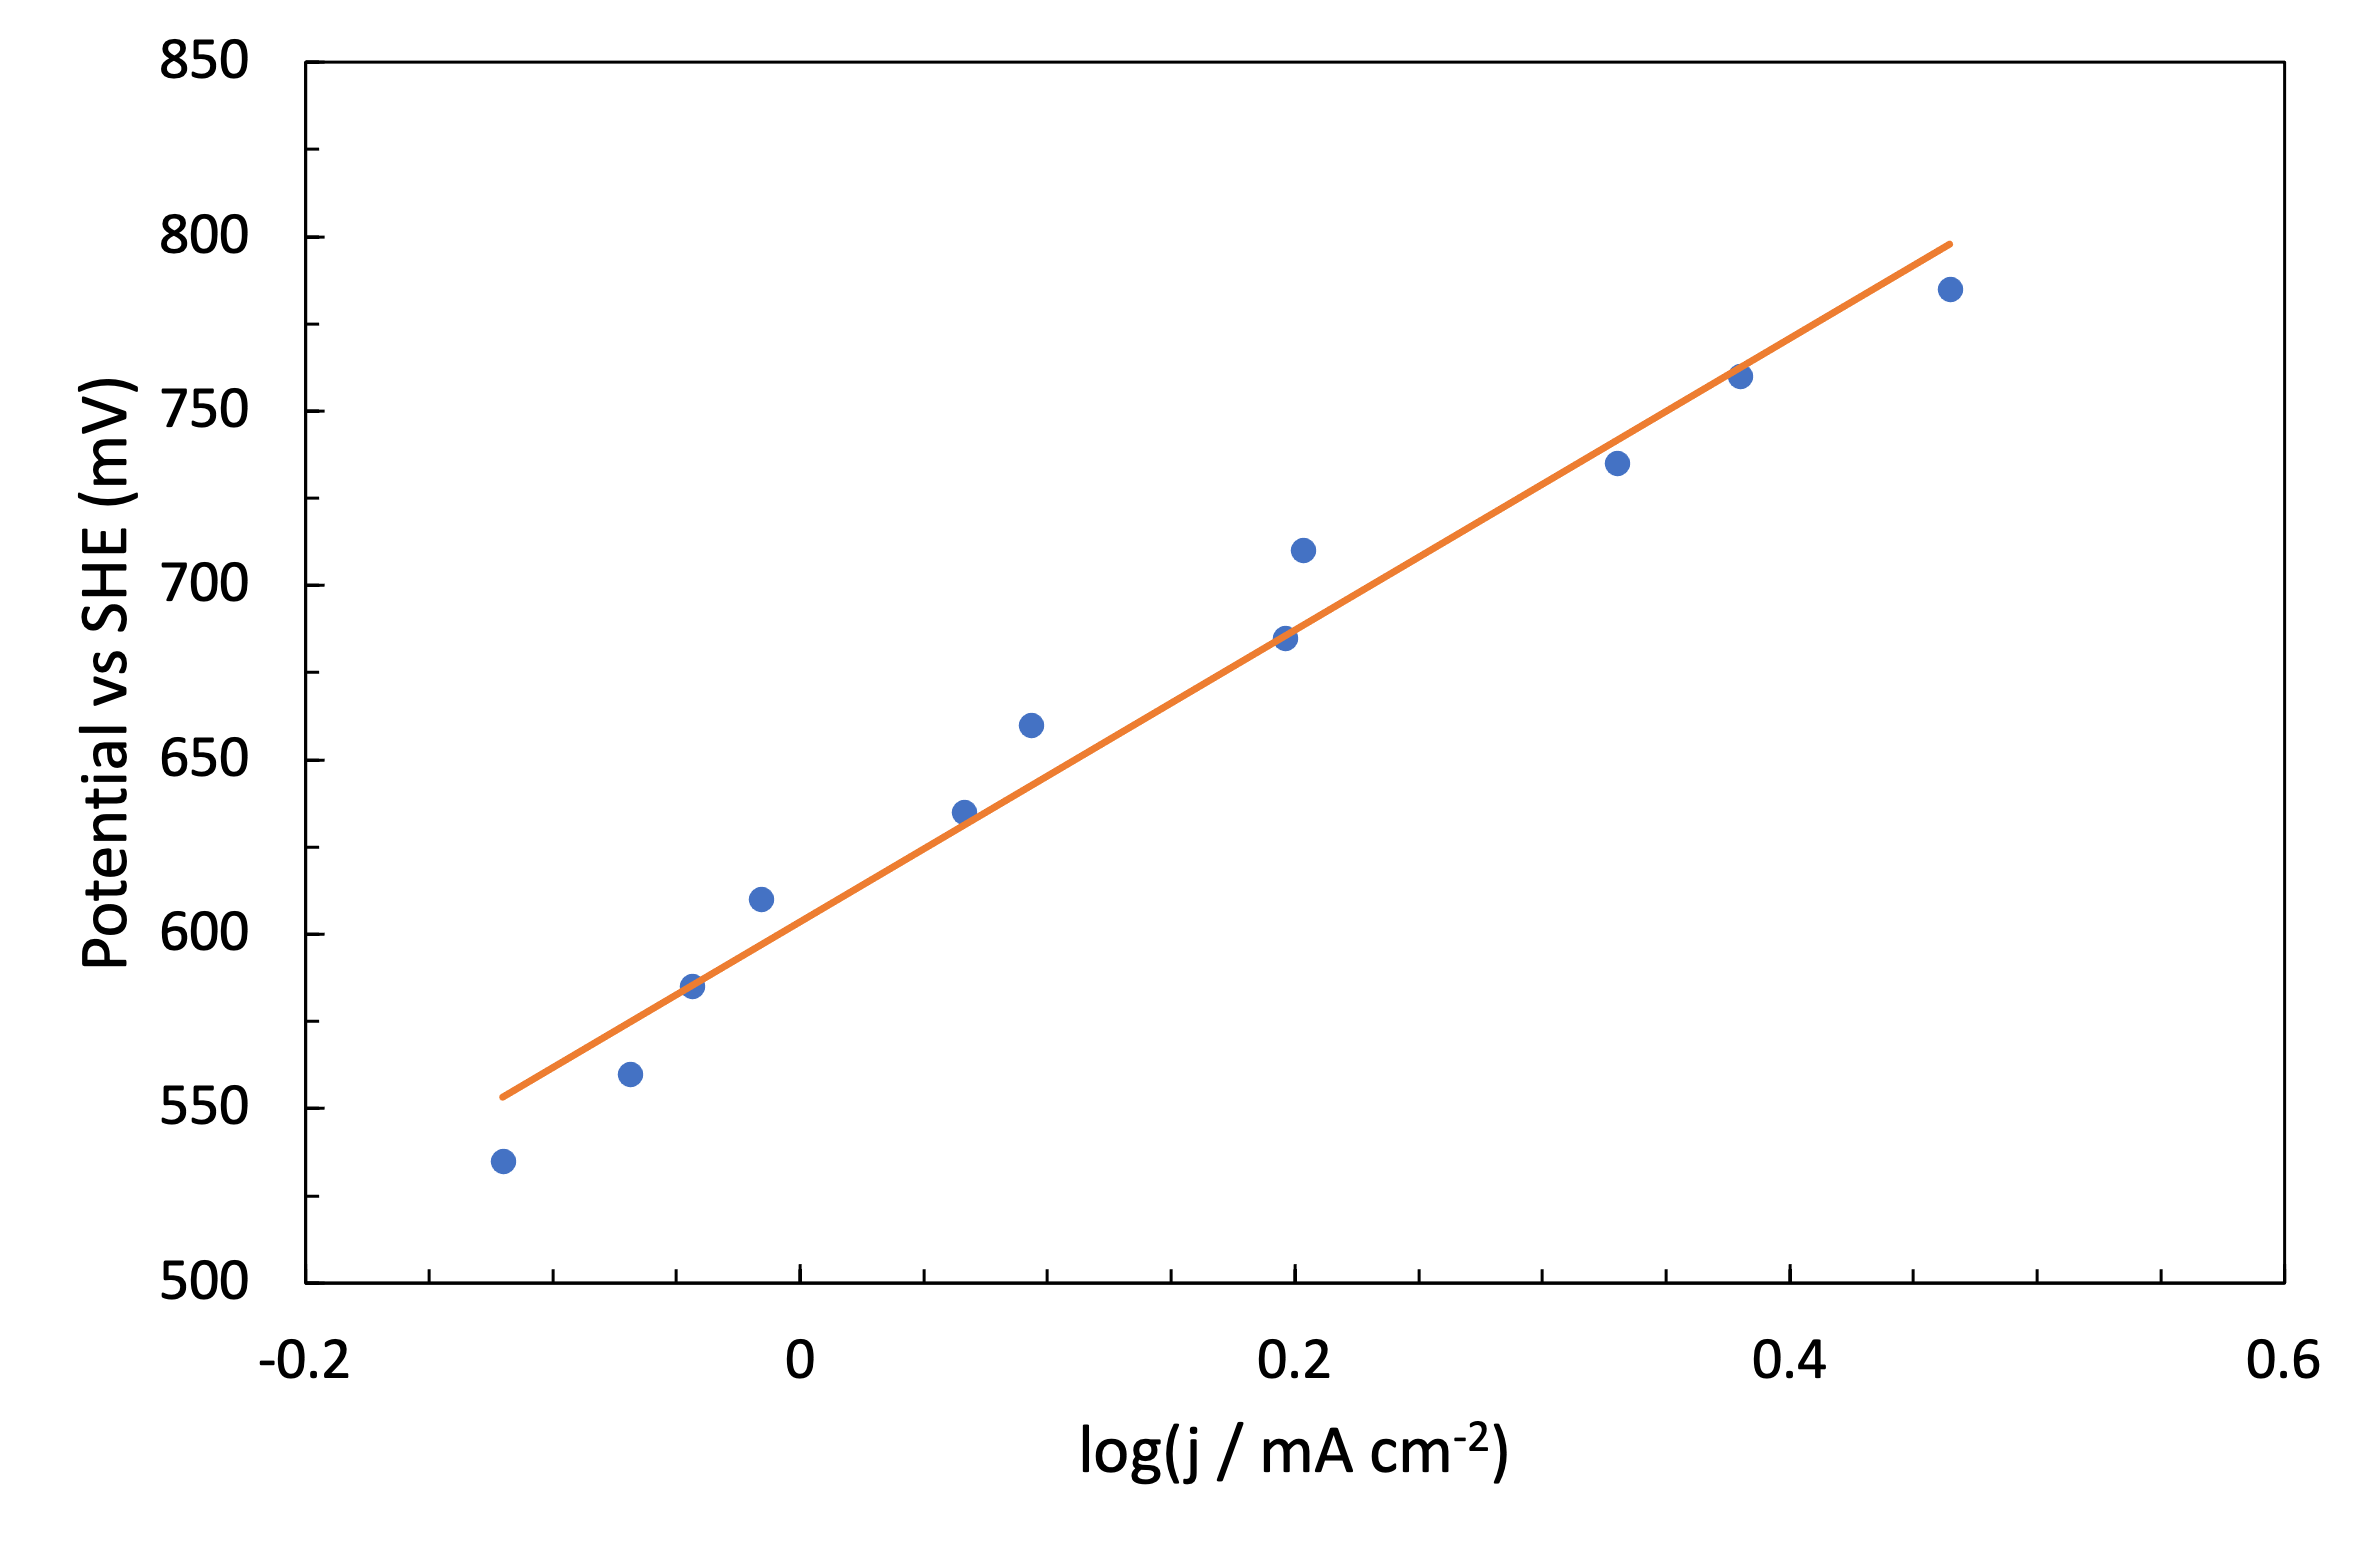
\includegraphics[width=0.95\linewidth]{lab5-CATi.png}
    \caption{Tafel plot for the HER over a \ce{Ti} electrode in \SI{0.1}{\molar} \ce{H2SO4}. The potentials (in \si{\volt}) were selected on the basis of preceding cyclic voltammetry experiments to surround the foot of the catalytic wave in \SI{25}{\milli\volt} intervals. The logarithmic current densities were calculated from the average current measured at each potential in the last \SI{30}{\second} of a \SI{100}{\second} cyclic amperometry experiment conducted at a given potential, and normalized using the platinum electrode surface area of \SI{0.63}{\centi\meter\squared}. Data analysis and linear regression was performed in Excel using the Solver function. A positive Tafel slope is observed: $m=\SI{402}{\milli\volt/dec}$ and $b=\SI{608}{\milli\volt}$ for a fit to $\eta=m\cdot\log(j)+b$.}
    \label{fig:CATi}
\end{figure}

The Tafel slopes for platinum and tin are different. In particular, the respective slopes are \SI{48}{\milli\volt/log(j)} and \SI{359}{\milli\volt/log(j)}. Comparing these values with the predicted Tafel slopes in the introduction reveals that platinum most likely proceeds via a V-T mechanism and thus exhibits an acid concentration dependence of 2, while tin most likely proceeds via a V-H mechanism and thus exhibits an acid concentration dependence of 1.\par
On rate laws, the above concentration dependence and Wuttig\supercite{bib:WuttigLecture} imply that
\begin{equation}
    R_{\ce{Pt}} = k_1[\ce{H3O+}]^2\e[-\beta\eta F/RT]
\end{equation}
and
\begin{equation}
    R_{\ce{Sn}} = k_2[\ce{H3O+}]\e[-\beta\eta F/RT]
\end{equation}
Lastly, it follows from the CV data (Figures \ref{fig:CVPtA}-\ref{fig:CVTiJ}) that the optimal binding energetics of the hydride intermediate should preferably be bound neither too tightly nor too loosely. This results in a "volcano plot" of transition metals, as seen in the lab manual\supercite{bib:LabManual2}.


\subsection*{Conclusion}
% This experiment utilized cyclic voltammetry and chronoamperometry to analyze a hydrogen evolution reaction using platinum, titanium, and tin electrodes as catalysts in an electrochemical cell with 0.1 M H2SO4 electrolyte solution. Using an SHE scale, the cyclic voltammetry data was plotted for both an unnormalized current and a current normalized by the geometric surface area of the electrodes. Normalizing for the geometric surface area accounted for the available surface atoms interacting with the solution on each electrode. The CV data indicated the catalytic abilities of each material for the HER reaction, as seen by the necessary overpotential. \par
% The onset potential was determined for each CV by analyzing the foot of the curve, denoting the start of the hydrogen evolution reaction. Multiple points above and below the onset potential were used in order to perform chronoamperometry. The CA data was used to plot a Tafel plot for each of the catalysts. The Solver Excel tool was used to determine the slope of the Tafel plots in order to collect data on the rate of the overpotential change per current density change. The slope of the Tafel plot could then be used to determine the mechanism behind each of the catalyst's HER reaction.\par
% It was concluded that the mechanism of the platinum catalyst HER reaction is the Volmer-Tafel mechanism while the mechanism of the titanium and tin catalysts is the Volmer-Heyrovsky mechanism based on the known slopes of the Tafel plots for each mechanism. The platinum electrode had a Tafel plot slope of 51.7 mV/log j, which is similar to the expected Volmer-Tafel slope of 30 mV/log j. The titanium and tin electrodes had Tafel plot slopes of 418 mV/log j and 359 mV/log j respectively, which is more similar to the expected Volmer-Heryovsky slope of 120 mV/log j. \par
% Multiple sources of error can be identified throughout this experiment that likely skewed the results. Corrosion and fragmentation of the electrodes, especially the tin electrode is one way in which the current could have been changed. The tin and titanium electrodes are also likely undergoing other reduction and oxidation reactions as seen by the peaks on the right hand side of the CV graphs. Both the tin and titanium electrodes are likely both being oxidized by oxygen as well as the surface metal oxide is likely reduced back into the non-oxidized species. Thus, the current data is not unique to just the HER reaction as assumed. The platinum electrode was also a higher professional grade as compared to the titanium and tin homemade electrodes. \par
% With respect to the binding energetics of the intermediates, the strength of the metal-hydride bond is an important indicator of the efficiency of the catalyst. The metal hydride bond strength must not be too strong as to inhibit the reaction while also not too weak as to not provide enough driving force. \par
% This experiment provided information about the catalytic capabilities of platinum, titanium, and tin and demonstrated that platinum is the most effective electrode to use as a catalyst for the HER reaction followed by titanium and then tin. The experiment also provided information about the rate and mechanism of the reaction as well as its dependence on the metal hydride bond strength. Overall, this experiment provides information about the factors to be considered when designing an efficient electrocatalyst. 

In this experiment, the onset potential was determined for each metal by finding the foot of the catalytic wave in the CV diagrams. This illustrated that \ce{Pt} was the most active electrocatalyst, followed by \ce{Ti} and then \ce{Sn}. The foot of the catalytic wave was also used to locate points for use in chronoamperometry with the goal of constructing a Tafel plot. Said plot enabled the determination of which reaction mechanism took place over each metal (specifically \ce{Pt} and \ce{Sn}). In particular, it was determined that \ce{Pt} makes use of the V-T mechanism while \ce{Sn} makes use of the V-H mechanism. Overall, the data suggested the strong role of metal-hydride binding energetics in determining catalytic efficiency and activity.\par
Throughout the experiment, several sources of error likely affected results. First off, corrosion and fragmentation of the tin electrode likely drastically affected its electrochemistry. In particular, some electrons likely went toward reducing the tin oxides created on the positive sweeps, increasing the measured current. This would have also lowered the Faradaic efficiency from 100\%, affecting some later calculations. Additionally, both the platinum and titanium electrodes likely undergo mild oxidation and corrosion, too, hence the requisite cleaning after each scan. Thus, the surface area is likely not constant throughout the reaction but would shrink, slightly raising the current density in later cycles. Moreover, normalization would need to be conducted in a more sophisticated manner. Furthermore, the tin and titanium electrodes were made in-house and not of the same professional caliber as the platinum electrode, so their more rudimentary form likely made the data collected on them generally less accurate as well. One last bit of experimental error is the aforementioned failure to stir the reaction during the platinum CA experiment likely made that data less than perfect, and extra cleaning of the cells between experiments would have made the data more accurate as well. On the analytical side, the models used generally gave interpretations of the data consistent with the theory. However, one particular place where they may be incomplete is indicated by the smoothness of the hypothetical curve connecting the data points in Figures \ref{fig:CVPtA}-\ref{fig:CVPtJ} and \ref{fig:CVSnA}-\ref{fig:CVSnJ}. That the curve would be so smooth is highly unlikely statistically, and likely suggests the presence of a higher level chemical process containing more relevant information that the simplistic linear regression used does not capture.\par
Altogether, the data herein provides insight into the catalytic mechanism of hydrogen evolution over potential electrocatalysts, confirming the strong ability of one particular material (platinum) to catalyze said reaction and making it easier to design future experiments regarding this critical clean energy tool.
\newpage


\printbibliography
\setcounter{figure}{0}
\setcounter{table}{0}




\end{document}